%%%%%%%%%%%%%%%%%%%%%%%%%%%%%%%%%%%%%%%%%%%%%%%%%%%%%%%%%%%%%%%%%%%%%%%%%%%%
% AGUtmpl.tex: this template file is for articles formatted with LaTeX2e,
% Modified July 2014
%
% This template includes commands and instructions
% given in the order necessary to produce a final output that will
% satisfy AGU requirements.
%
% PLEASE DO NOT USE YOUR OWN MACROS
% DO NOT USE \newcommand, \renewcommand, or \def.
%
% FOR FIGURES, DO NOT USE \psfrag or \subfigure.
%
%%%%%%%%%%%%%%%%%%%%%%%%%%%%%%%%%%%%%%%%%%%%%%%%%%%%%%%%%%%%%%%%%%%%%%%%%%%%
%
% All questions should be e-mailed to latex@agu.org.
%
%%%%%%%%%%%%%%%%%%%%%%%%%%%%%%%%%%%%%%%%%%%%%%%%%%%%%%%%%%%%%%%%%%%%%%%%%%%%
%
% Step 1: Set the \documentclass
%
% There are two options for article format: two column (default)
% and draft.
%
% PLEASE USE THE DRAFT OPTION TO SUBMIT YOUR PAPERS.
% The draft option produces double spaced output.
%
% Choose the journal abbreviation for the journal you are
% submitting to:

% jgrga JOURNAL OF GEOPHYSICAL RESEARCH
% gbc   GLOBAL BIOCHEMICAL CYCLES
% grl   GEOPHYSICAL RESEARCH LETTERS
% pal   PALEOCEANOGRAPHY
% ras   RADIO SCIENCE
% rog   REVIEWS OF GEOPHYSICS
% tec   TECTONICS
% wrr   WATER RESOURCES RESEARCH
% gc    GEOCHEMISTRY, GEOPHYSICS, GEOSYSTEMS
% sw    SPACE WEATHER
% ms    JAMES
% ef    EARTH'S FUTURE
% ea    EARTH AND SPACE SCIENCE
%
%
%
% (If you are submitting to a journal other than jgrga,
% substitute the initials of the journal for "jgrga" below.)

\documentclass[draft,ms]{agutex}   %draft, [ms]
% To create numbered lines:

% If you don't already have lineno.sty, you can download it from
% http://www.ctan.org/tex-archive/macros/latex/contrib/ednotes/
% (or search the internet for lineno.sty ctan), available at TeX Archive Network (CTAN).
% Take care that you always use the latest version.

% To activate the commands, uncomment \usepackage{lineno}
% and \linenumbers*[1]command, below:

\usepackage{lineno}
\linenumbers*[1]
%  To add line numbers to lines with equations:
%  \begin{linenomath*}
%  \begin{equation}
%  \end{equation}
%  \end{linenomath*}
%%%%%%%%%%%%%%%%%%%%%%%%%%%%%%%%%%%%%%%%%%%%%%%%%%%%%%%%%%%%%%%%%%%%%%%%%
\usepackage{url}
\usepackage{amsmath}
\usepackage{rotating} 

\usepackage[bottom]{footmisc}

\usepackage{graphics}

%\usepackage[dvips]{graphicx}
 
\usepackage{color}
\definecolor{pinkred}{rgb}{1.0, 0.4, 0.4}
\usepackage[table]{xcolor}

% Author names in capital letters:
\authorrunninghead{HUANG ET AL.}

% Shorter version of title entered in capital letters:
\titlerunninghead{EVALUATION OF VR-CESM FOR MODELING CALIFORNIA'S CLIMATE}

%Corresponding author mailing address and e-mail address:
\authoraddr{Corresponding author: Xingying Huang,
Department of Land, Air and Water Resources, \\
 University of California Davis, Davis, CA 95616, USA.
 (xyhuang@ucdavis.edu)}
 
%Department of Hydrology and Water Resources, University of
%Arizona, Harshbarger Building 11, Tucson, AZ 85721, USA.
%(a.b.smith@hwr.arizona.edu)}

\begin{document}

%% ------------------------------------------------------------------------ %%
%
%  TITLE
%
%% ------------------------------------------------------------------------ %%


\title{An Evaluation of the Variable Resolution-CESM for Modeling California's Climate}

    \authors{Xingying Huang,\altaffilmark{1}
  Alan M. Rhoades, \altaffilmark{1} Paul A. Ullrich, \altaffilmark{1} 
  Colin M. Zarzycki, \altaffilmark{2}}

\altaffiltext{1}{Department of Land, Air and Water Resources, University of California, Davis}
\altaffiltext{2}{National Center for Atmospheric Research}


%%%%%%%%%%%%%%%%%%%%%%%%%%%%%%%%%%%%%%%%%%%%%%%%%%%%%%%%%%%%%%%%%%%%%
% ABSTRACT
%
% Enter your Abstract here

\begin{abstract}

In this paper the recently developed variable-resolution option within the Community Earth System Model (VR-CESM) is assessed for long-term regional climate modeling of California at $\sim$28 km and $\sim$14 km horizontal resolutions. The mean climatology of near-surface temperature and precipitation is analyzed and contrasted with reanalysis, gridded observational datasets and a traditional regional climate model (RCM) -- the Weather Research and Forcasting (WRF) model. Statistical metrics for model evaluation and tests for differential significance have been extensively applied. With only prescribed sea surface temperatures, VR-CESM tended to produce a warmer summer (by about 1 to 3 $^\circ$C) and overestimated overall winter precipitation (about 25$\%$-35$\%$) compared to reference datasets. Increasing resolution from 28 km to 14 km did not produce a statistically significant improvement in the model results. By comparison, the analogous WRF climatology (constrained laterally and at the sea surface by ERA-Interim reanalysis) was $\sim$1 to 3 $^\circ$C colder than the reference datasets, underestimated precipitation by $\sim$20$\%$-30$\%$ at 27 km resolution and overestimated precipitation by $\sim$65-85$\%$ at 9 km.  Overall, VR-CESM produced comparable statistical biases to WRF in key climatological quantities.  This assessment highlights the value of variable-resolution global climate models (VRGCMs) in capturing fine-scale atmospheric processes, projecting future regional climate and addressing the computational expense of uniform-resolution global climate models.

\end{abstract} 

\begin{article}

%%%%%%%%%%%%%%%%%%%%%%%%%%%%%%%%%%%%%%%%%%%%%%%%%%%%%%%%%%%%%%%%%%%%%
% MAIN BODY OF PAPER
%%%%%%%%%%%%%%%%%%%%%%%%%%%%%%%%%%%%%%%%%%%%%%%%%%%%%%%%%%%%%%%%%%%%%
%
\section{Introduction}

Global climate models (GCMs) have been widely used to simulate both past and future climate. Although these models have demonstrable success in representing large-scale features of the climate system, they are usually employed at relatively coarse resolutions ($\sim$1$^\circ$), largely as a result of the substantial computational cost required at higher resolutions. Global climate reanalysis datasets, which assimilate climate observations using a global model, represent a best estimate of historical weather patterns. However, reanalysis datasets still cannot fulfill the needs of policymakers, stakeholders and researchers that require high-resolution regional climate data (\url{http://reanalyses.org/atmosphere/overview-current-reanalyses}). Regional features such as microclimates, land cover, and topography, are not well captured by either GCMs or reanalysis datasets \citep{leung2003regional}.  However, dynamical processes at unrepresented scales are significant drivers for local climate variability, especially over complex terrain \citep{soares2012wrf}. In order to capture fine-scale dynamical features, high horizontal resolution is needed for a more accurate representation of small-scale processes and interactions \citep{rauscher2010resolution}. With these enhancements, regional climate data is expected to be more useful for formulating climate adaptation and mitigation strategies locally.

In order to model regional climate at high spatial resolutions over a limited area, downscaling techniques have been developed, such as statistical and dynamical downscaling. Dynamical downscaling typically uses nested limited-area models (LAMs) or, more recently, variable-resolution enabled GCMs (VRGCMs) \citep{laprise2008regional}. In this context, LAMs are typically referred to as regional climate models (RCMs) when used for climate study. Forced by the output from GCMs or reanalysis datasets, RCMs have been widely used to capture physically consistent regional and local circulations at the needed spatial and temporal scales \citep{christensen2007regional, bukovsky2009precipitation, mearns2012north}. Recently, there has been a growing interests in the use of VRGCMs for modeling regional climate. Unlike RCMs, VRGCMs use a relatively coarse global model with enhanced resolution over a specific region \citep{staniforth1978variable, fox1997finite}.  Strategies that have been employed for transitioning between coarse and fine-resolution regions within a VRGCM include grid stretching \citep{fox1997finite, mcgregor2008updated} and grid refinement \citep{ringler2008multiresolution, skamarock2012multiscale, zarzycki2014aquaplanet}. VRGCMs have demonstrated utility for regional climate studies and applications at a reduced computational cost compared to uniform GCMs \citep{fox2006variable, rauscher2013exploring, zarzycki2015effects}. 

Compared with RCMs, a key advantage of VRGCMs is that they use a single, unified modeling framework, rather than two separate models (GCM and RCM) with potentially disparate dynamics and physics parameterizations. RCMs may suffer from potential inconsistencies between the global and regional scales and lack two-way interactions at the nest boundary \citep{warner1997tutorial, mcdonald2003transparent, laprise2008challenging, mesinger2013limited}, which can be mitigated with the use of VRGCMs. VRGCMs also provide a cost-effective method of reaching high resolutions over a region of interest -- the limited area simulations in this study at 0.25$^\circ$ and 0.125$^\circ$ resolution represent a reduction in required computation of approximately 10 and 25 times, respectively, compared to analogous globally uniform high-resolution simulations. For the purposes of this paper, we focus on the recently developed Community Earth System Model with variable-resolution option (VR-CESM) as our VRGCM of interest. This configuration is driven by the Community Atmosphere Model's (CAM's) Spectral Element (SE) dynamical core, which possesses attractive conservation and parallel scaling properties \citep{dennis2011cam, taylor2011conservation}, as well as recently developed variable-resolution capabilities \citep{zarzycki2014aquaplanet, zarzycki2015experimental}. This model has been employed by \cite{zarzycki2014using} to show that a high-resolution refinement patch in the Atlantic basin for simulating topical cyclones represented significant improvements over the unrefined simulation. \cite{zarzycki2015effects} also compared the large-scale climatology of VR-CESM 0.25$^\circ$ and uniform CESM at 1$^\circ$, and found that adding a refined region over the globe did not noticeably affect the global circulation. \cite{rhoades2015characterizing} has also assessed the use of VR-CESM for modeling Sierra Nevada mountain snowpack in the western United States.


However, for the purposes of long-term regional climate modeling, particularly in regions where high-resolution is anticipated to be most beneficial, VR-CESM has yet to be rigorously evaluated. This paper aims to fill that gap by analyzing the performance of VR-CESM against gridded observational data, reanalysis product and in comparison to a traditional RCM forced by reanalysis data. Our variable-resolution simulations are implemented with horizontal resolutions of 0.25$^\circ$ and 0.125$^\circ$ respectively, which are much more typical for dynamically downscaled studies. This paper focuses on California in the western United States as the study area. The complex topography and coastlines of California strongly modulate large-scale weather patterns, creating local climatic features such as coastal fog, sea breeze, mountain-induced precipitation and snowpack. An understanding of local climate variability in California is incredibly important for policymakers and stakeholders due to its vast agricultural industry, mixed demographics, and vulnerability to anthropogenically-induced climate change \citep{hayhoe2004emissions, cayan2008overview}.  Consequently, we expect that California is an excellent test bed for regional climate modeling.


In this study the Weather Research and Forecasting (WRF, \cite{skamarock2005coauthors}) model has been used for simulating California's climatology at 27km and 9km grid spacing. RCM simulations over California have also been conducted in previous studies and demonstrated the need for high spatial and temporal resolution to better address regional climate and extreme events, especially in the vicinity of complex topography where large climatological gradients are present \citep{leung2004mid, kanamitsu2007fifty, caldwell2009evaluation, pan2011influences, pierce2013probabilistic}. In particular, \cite{caldwell2009evaluation} presented results from WRF at 12km spatial resolution and showed that, although the RCM was effective at simulating the mean climate when compared with observations, some clear biases persisted (particularly an overestimation of precipitation).

This study focuses on the models' ability to represent current climate statistics, particularly those relevant to heat and precipitation extremes. We anticipate that this work will validate VR-CESM for modeling the mean regional climatology of California and will further motivate the adoption of variable-resolution modeling to study other local climatic processes. Our eventual goal is to utilize these models for assessing historical and future regional climate extremes.


This paper is organized as follows: Section 2 describes the model setup, datasets and methodology for evaluation and intercomparison. In section 3, simulation results are provided and discussed, with focuses on near-surface (2-meter) temperature and precipitation. Key results are summarized along with further discussion in section 4.


\section{Models and Methodology}

\subsection{Simulation design} 

In this study, all global simulations use the Atmospheric Model Intercomparison Project (AMIP) experimental protocols \citep{Gates1992}. These protocols are widely used and support climate model diagnosis, validation and intercomparison. AMIP experiments are constrained by realistic sea-surface temperatures (SSTs) and sea ice from 1979 to near present without the added complexity of ocean-atmosphere feedbacks in the climate system. In particular, observed SSTs and sea ice at 1$^\circ$ horizontal resolution are provided and updated following the procedure described by \citep{hurrell2008new}.

\subsubsection{VR-CESM}

CESM is a state-of-the-art Earth modeling framework managed by the National Center for Atmospheric Research (NCAR), consisting of coupled atmospheric, oceanic, land and sea ice models.  For decades CESM (and its predecessor, the Community Climate System Model) has been used for modeling present and future global climate \citep{neale2010description, hurrell2013community}.  The coupling infrastructure in CESM communicates the interfacial states and fluxes between each component model to ensure conservation. Since we follow AMIP protocols, only the atmosphere and land model are integrated dynamically. Here, CAM version 5 (CAM5) \citep{CAM5Tech} and the Community Land Model (CLM) version 4.0 \citep{CLM40Tech} are used. As mentioned earlier, the SE dynamical core is employed along with variable-resolution grid support. The FAMIPC5 (F$\_$AMIP$\_$CAM5) component set, which mainly supports atmospheric, oceanic, land and sea ice models, is chosen for these simulations. In CAM5, cloud microphysics is parameterized using the two-moment scheme with with ice supersaturation \citep{ morrison2008new, gettelman2008new}, and the deep convection process is treated by Zhang and McFarlane (ZM) cumulus scheme \citep{zhang1995sensitivity}. A more detailed discussion of the CAM5 configuration can be found in \citep{neale2010description}.

For our study, the variable-resolution cubed-sphere grids are generated for use in CAM and CLM with the open-source software package SQuadGen \citep{ullrich2014squadgen,guba2014spectral}. The grids used in this study are depicted in Figure \ref{fig:Figure 1}.  The maximum horizontal resolution on these grids is 0.25$^\circ$ ($\sim$28km) and 0.125$^\circ$ ($\sim$14km) respectively, with a quasi-uniform 1$^\circ$ mesh over the remainder of the globe. Grids are constructed using a paving technique with a 2:1 spatial resolution ratio, so two transition layers are required from 1$^\circ$ to 0.25$^\circ$, and one additional transition from 0.25$^\circ$ to 0.125$^\circ$. In our study, and previous studies (e.g. \cite{zarzycki2015effects}), general circulation patterns (e.g., wind, pressure and precipitation) do not exhibit apparent artifacts in the variable-resolution transition region, and the design of the SE dynamical core ensures that dry air and tracer mass are conserved globally \citep{taylor2010compatible}. Simulations are performed over the time period from 1979-01-01 to 2005-12-31 (UTC) and year 1979 is discarded as a spin-up period. This 26-year time period is chosen to provide an adequate sampling of inter-annual variability, to limit computational cost, and to coincide with the satellite era where adequate high-quality gridded and reanalysis datasets are available.

Variable-resolution topography files were produced by sampling the National Geophysical Data Center (NGDC) 2-min ($\sim$4 km) Gridded Global Relief Dataset (ETOPO2v2), followed by the application of a differential smoothing technique as described in \cite{zarzycki2015effects}.  Using this technique, the $c$ parameter from their Eq. (1) was adjusted to reduce noise in the vertical pressure velocity field. The grid-scale topography is depicted in Figure \ref{fig:Figure 2}, including the topography of uniform CESM at 1$^\circ$ and observed topography from USGS 2 minute (~3 km) dataset. The hypsometric curves, showing the percentage of the Earth's surface above specific elevation, are also depicted for the models and observations (see Figure \ref{fig:Figure 2}). As we can see, higher resolution provides clear improvement in the representation of regional topography, which is necessary for the correct treatment of fine-scale dynamic processes strongly influenced by complex terrain. In the aspect of topography, WRF 9km is most closest to USGS dataset, while WRF 27km and VR-CESM 0.125$^\circ$ are quite similar to each other. Topography at very coarse resolution ($\sim$1$^\circ$) is too smooth to represent local details like the shape of valleys or mountain peaks, resulting in the loss of regional climate patterns.

Land surface datasets, including plant functional types, at $0.5$$^\circ$ were adopted. Greenhouse gas (GHG) concentrations and aerosol forcings are prescribed based on historical observations. CAM and CLM tuning parameters are not modified from their default configurations.


\subsubsection{WRF} 

WRF has been widely used over the past decade for modeling regional climate \citep{lo2008assessment, leung2009atmospheric, soares2012wrf, sun2015hybrid}. In our study, the fully compressible non-hydrostatic WRF model (version 3.5.1) with the Advanced Research WRF (ARW) dynamical core is used.  WRF is a limited area model that supports nested domains with a typical refinement ratio of 3:1.  The simulation domains of WRF are depicted in Figure \ref{fig:Figure 3}. Two WRF simulations, representing finest grid resolutions of 27 km and 9 km, are conducted.  For the WRF 27km simulation, one domain is used. For the WRF 9km simulation, two domains are used, with the outer domain at 27 km (same as the WRF 27km) and an inner nested domain at 9 km horizontal grid resolution. For both simulations,  grids are centered on California and have 120$\times$110 and 151$\times$172 grid points, respectively. At all lateral boundaries, 10 grid points are used for relaxation to the coarse solution. In order to reduce the drift between forcing data and modeling output, grid nudging \citep{stauffer1990use} is applied to the outer domain every 6 hours at all levels except approximate planetary boundary layers (PBL), as suggested by \cite{lo2008assessment}. The nudging is applied to the wind, temperature and water vapor mixing ratio with default nudging coefficients. Grid nudging is commonly used and maturely supported in WRF. Although there is evidence spectral nudging may improve the quality of the simulations, an investigation of these differences is out of scope for this paper \citep{liu2012differences}. This setup uses 41 vertical levels with model top pressure at 50 hPa.

Additionally, the following physics parameterizations are employed: WSM (WRF Single-Moment) 6-class graupel microphysics scheme \citep{hong2006wrf}, Kain-Fritsch cumulus scheme \citep{kain2004kain}, CAM shortwave and longwave radiation schemes \citep{collins2004description}.  These settings are chosen by assessing the results from several common parameterization combinations over one-year simulation, with comparing to gridded observations. For the boundary layer, the Yonsei University scheme (YSU) \citep{hong2006new} is used, and the Noah Land Surface Model \citep{chen2001coupling} is applied. Both are chosen as they are common for climate applications that balance long-term reliability and computational cost.  Although many other options and combinations of parameterizations are available for configuring WRF (and others have tackled a complete assessment of these options for particular problems), our choices are made simply to represent a typical WRF configuration. We do note that the Kain-Fritsch convective parameterization remains active even in the 9km inner mesh -- although this is considered within the ``gray zone'', it had no appreciable impact on the simulation since almost all precipitation emerged from (large-scale) condensation, as discussed in Section 4.

ECMWF Reanalysis (ERA-Interim) data at both the surface and multiple pressure-levels provides initial and lateral conditions for the domains. The lateral conditions and SSTs are updated every 6 hours. ERA-Interim reanalysis ($\sim$80 km) has been widely used and validated for its reliability as forcing data \citep{dee2011era}. WRF simulations are conducted over the same time period as VR-CESM (i.e., 1979-01-01 through 2005-12-31 UTC). Again, the year 1979 is used as a spin-up period and is discarded for purposes of analysis. Notably, the $\sim$9 km resolution employed in the innermost domain is finer than most previous studies for long-term climate.

The topography employed for the 27 km and 9 km simulations is interpolated from USGS (United States Geological Survey) elevation data with 10-min ($\sim$20 km) and 2-min ($\sim$4 km) resolution, respectively. The post-processed grid-scale topography is contrasted in Figure \ref{fig:Figure 2}. Elevation differences between VR-CESM and WRF are irregular and relatively small, except over the Central Valley where VR-CESM has consistently higher values than WRF. This indicates a different methodology for preparation of the topography dataset and may also be partly due to the use of the USGS elevation instead of NGDC elevation datasets. 

\subsection{Gridded and Reanalysis Datasets}

Reanalysis and gridded observational datasets of the highest available quality are employed (see Table \ref{tab:Datasets}). Differences between gridded observations can be due to the choice of meteorological stations, interpolation techniques, elevation models and processing algorithms.  Consequently, the use of multiple reference datasets is necessary to understand the underlying uncertainty in the observational data.  Detailed descriptions of these datasets are as follows.

\paragraph{NARR}  The North American Regional Reanalysis (NARR) is the NCEP (National Centers for Environmental Prediction) high-resolution reanalysis product that provides dynamically downscaled data over North America at $\sim$32 km resolution and 3-hourly intervals from 1979 through present \citep{mesinger2006north}. We note that some inaccuracies have also been identified in NARR, particularly in precipitation fields \citep{bukovsky2007brief}.

\paragraph{NCEP CPC} This dataset provides gauge-based analysis of daily precipitation from the National Oceanic and Atmospheric Administration (NOAA) Climate Prediction Center (CPC). It is a suite of unified precipitation products obtained by combining all information available at CPC via the optimal interpolation objective analysis technique. The gauge analysis covers the Conterminous United States with a fine-resolution at 0.25$^\circ$ from 1948-01-01 to 2006-12-31.


\paragraph{PRISM} The Parameter-elevation Regressions on Independent Slopes Model (PRISM) \citep{daly2008physiographically} supports a 4 km gridded dataset obtained by taking point measurements and applying a weighted regression scheme that accounts for many factors affecting the local climatology. The datasets include total precipitation and minimum/maximum, (derived) mean temperatures and dewpoints. Monthly climatological variables are available for 1895 through 2014 from the PRISM Climate Group (Oregon State University, \url{http://prism.oregonstate.edu}, created 4 Feb 2004). Notably, PRISM is the United States Department of Agriculture's official climatological dataset.  PRISM is used as our primary reference dataset for model performance evaluation.

\paragraph{UW} The UW daily gridded meteorological data is obtained from the Surface Water Modeling group at the University of Washington \citep{maurer2002long, hamlet2005production}. UW incorporates topographic corrections by forcing the long-term average precipitation to match that of the PRISM dataset. The temperature dataset is produced in a similar fashion as precipitation, but uses a simple 6.1 K/km lapse rate for topographic effect. The dataset is provided at 0.125$^\circ$ horizontal resolution covering the period 1949 to 2010.


\paragraph{Daymet}  Daymet is an extremely high resolution (1 km) gridded dataset with daily outputs of total precipitation, humidity, and minimum/maximum temperature covering 1980 through 2013 \citep{thornton1997generating, thornton2014daymet}. The dataset is produced using an algorithmic technique that ingests point station measurements in conjunction with a truncated Gaussian weighting filter.  Some adjustments are made to account for topography. Daymet is available through the Oak Ridge National Laboratory Distributed Active Archive Center (ORNL DAAC). 

To assess differences in these data products, we have calculated the MSD values among PRISM, UW and Daymet for seasonally averaged JJA T$_{max}$, T$_{min}$ and DJF Pr over the five divisions and tabulated these results in Table \ref{tab:stat_Datasets}. Student's t-test is employed to determine significances of differences. For T$_{max}$ and T$_{min}$, gridded observational datasets are different from each other over some divisions.  The most pronounced divergences occur in the NC region, with MSD values reaching up to $\sim$4$^\circ$C, although differences are also apparent for MR T$_{min}$. Clearly, UW and Daymet have a colder climatology than PRISM. NARR, as a reanalysis dataset, is different from the others over most divisions, with overall larger T$_{min}$ and smaller T$_{max}$. For precipitation, essentially no significant differences are present, especially among PRISM, UW and Daymet. NARR and CPC (not shown) seem to have slightly lower precipitation values than others.

\subsection{Methodology}

Near-surface temperature and precipitation have been analyzed over California to assess the performance of VR-CESM in representing the mean climatology. Specifically, our evaluation focuses on daily maximum, minimum and average near-surface temperatures (T$_{max}$, T$_{min}$ and T$_{avg}$) and daily precipitation (Pr). These variables are key in a baseline climate assessment due to their close relationship with water resources, agriculture and health. In this context, the biggest impact of weather on California is through heat and precipitation extremes. Since heat extremes dominate during the summer season, we focus on June, July and August (JJA) for assessment of temperature. On the other hand, since the vast majority of precipitation in California occurs in the winter season, December-January-February (DJF) is emphasized.  

In order to adequately account for natural variability of the mean climate, the simulation period must be chosen appropriately \citep{solomon2007climate}. However, the number of simulated years required for adequate climate statistics depends greatly on the regional climate variability and spatial scale. Past studies have used average weather conditions over a 30-year period to ensure sufficient statistics and to avoid imprinting from annual variability \citep{dinse2009climate}. To check that our 26-year simulation period is sufficient, we have examined the interannual variability of mean temperature and precipitation in all simulations and observations over 5, 10, 20 and 25 seasons or years (depicted in the supplemental figures). We observe that for climatological mean temperature and precipitation, the relevant statistics are effectively converged for a 20-year sample, suggesting that our simulation period is sufficient to adequately capture the interannual variability of these quantities. 


The results in section 4 are obtained from simulated and observed data over the period 1980 to 2005.  All datasets have been linearly de-trended at each grid point so as to facilitate averaging of all simulation years. It is found that, for annual and JJA near-surface temperature (T$_{max}$, T$_{min}$ and T$_{avg}$), a statistically significant trend is present under the two-tailed t-statistic with a significance level of 0.05. For T$_{min}$, the average warming in 26 years is $\sim$0.6 K$-$1 K for observations, $\sim$0.5 K for VR-CESMs and WRF 27km and $\sim$1.5 K for WRF 9km. For T$_{max}$, the average warming is $\sim$0.3 K$-$0.5 K for observations, $\sim$0.5 K$-$0.8 K for VR-CESMs and WRFs. No statistically significant trend has been detected for precipitation.

California consists of a diverse variety of climate regions as a consequence of its rugged topography and large latitudinal extent.  The distinct character of these regions is poorly captured in typical coarse global climate simulations \citep{abatzoglou2009classification, caldwell2009evaluation}.  In order to assess the performance of VR-CESM within each region, the state has been divided into five climate divisions, including the Central Valley (CV), Mountain Region (MR), North Coast (NC), South Coast (SC), and Desert Region (DR).  The spatial extent of these divisions is depicted in Figure \ref{fig:Figure 3}. These five divisions are determined loosely based on the results of \cite{abatzoglou2009classification} and the climate divisions used by the California Energy Commission. To restrict the analysis in each division, simulations and datasets have been masked to restrict climate variables to each division. 


Standard statistical measures have been used to quantify the model performance in comparison with the reference datasets. These include the root-mean-square deviation (RMSD), mean signed difference (MSD), mean relative absolute difference (MRD), and sample standard deviation ($s$). Further, spatial correlation is assessed by computing Pearson product-moment coefficient of linear correlation between climatological means from models and reference datasets.  Mathematically, these quantities are written as
\begin{align}
RMSD &= \sqrt{\frac{1}{N} \sum_{i=1}^{N} (v_i - \hat{v}_i)^2}  & MSD &= \frac{1}{N} \sum_{i=1}^{N} (v_i - \hat{v}_i) \\[2.0ex]
s &= \sqrt{\frac{1}{M-1} \sum_{j=1}^{M} (v_j - \bar{v})^2}   & MRD &= \left( \sum_{i=1}^{N} |v_i - \hat{v}_i| \right) \Bigg/ \left( \sum_{i=1}^{N} \hat{v}_i \right).
\end{align} where $v_i$ and $\hat{v}_i$ are values from the simulation output and reference dataset, respectively; $i$ is the grid-point index and N is the total number of grid points over specific regions; $j$ is the simulation year index, M is the total number of simulated years and $\bar{v}$ is the mean value over all years. Grid-point differences are calculated by remapping the reference datasets to the model's output grid using bilinear interpolation.  Remapping using patch-based interpolation has also been tested and nearly identical results have been observed.  When necessary, the statistical quantities are further averaged over each division.


Throughout the remainder of this paper, student's t-test has been used to test whether two sets of annual-, seasonal- or monthly-averaged data are the same. F-test is applied to test whether the sample variances are equal. These tests are used only when the sample population can be described adequately by a normal distribution, where normality is assessed under the Anderson-Darling test. When the sample populations do not approximately follow a normal distribution, Mann-Whitney-Wilcoxon (MWW) test and Levene's test are employed in lieu of the t-test and F-test, respectively. All statistical tests are evaluated at the $p = 0.05$ significance level.

Complementary results to this study are provided in the online supplement, including the original grid-refined mesh files, the sensitivity of climatological statistics to choice of time period, the observed time trend, and other seasons not addressed in this paper and corresponding statistics metric tables. Results are also provided with comparison of VR-CESM to the output from a globally uniform CESM run at 0.25$^\circ$ spatial resolution with the finite volume (FV) dynamical core \citep{wehner2014effect}.

\section{Results}

A detailed analysis of temperature and precipitation results from WRF and VR-CESM is provided in this section.  A concise summary of key points follows in section \ref{sec:Discussion}.

\subsection{Temperature}

The mean JJA T$_{max}$, T$_{min}$ and T$_{avg}$ climatology over the simulation period, together with PRISM and NARR reference data, is plotted in Figure \ref{fig:Figure 4}. UW and Daymet have not been plotted here since they are visually indistinguishable to PRISM everywhere except for NC, where UW and Daymet exhibit lower temperatures (see Table \ref{tab:stat_Datasets}).  Statistical measures over California are tabulated in Table \ref{tab:stat_JJA_t2}. In general, all simulations have captured the spatial climate patterns exhibited by PRISM, with high spatial correlations ($>$0.95), especially for T$_{max}$ and T$_{avg}$.  Nonetheless, several clear biases (relative to PRISM) are present in these simulations, as discussed below.

\begin{itemize}
\item{} \textbf{T$_{max}$:}  When compared with the reference datasets, VR-CESM showed a warm bias of about 2 to 3 $^\circ$C in T$_{max}$ over much of the inland domain (CV and MR) and a 2 to 3 $^\circ$C cool bias along the coast, although the coastal bias is reduced by $\sim$0.5 $^\circ$C at 0.125$^\circ$ resolution. This is in contrast with WRF, which produced an overall colder climate everywhere except the CV.  This bias is especially pronounced for the WRF 9km simulation, which was approximately 3 $^\circ$C cooler than PRISM. T$_{max}$ within the CV has been overestimated by all the simulations. This likely represents a systematic issue with high-resolution models with respect to California.  Possible reasons for this overestimation are discussed at the end of this section.


\item{} \textbf{T$_{min}$:}  VR-CESM showed a strong warm bias in T$_{min}$ ($\sim$2 to 4 $^\circ$C), with a particularly large overestimation over Nevada ($> 5 ^\circ$C). WRF also exhibited a warm bias, but of a much smaller magnitude ($\sim$2 to 3 $^\circ$C). However, the pattern of T$_{min}$ presented in Figure \ref{fig:Figure 4} in both WRF simulations suggests a cooler interior to the CV and warmer perimeter, which is not supported by observations.

\item{} \textbf{T$_{avg}$:}  The warm bias of T$_{min}$ and T$_{max}$ by VR-CESM resulted in a similar overestimation of T$_{avg}$. For WRF, underestimation of T$_{max}$ and overestimation of T$_{min}$ led to an overall closer match to T$_{avg}$ over most of the domain, but is indicative of a suppressed diurnal cycle.
\end{itemize}

Compared with the reference datasets over California, VR-CESM 0.125$^\circ$ produced the lowest RMSD values for T$_{max}$, whereas WRF had smallest RMSD for T$_{min}$.  However, in both cases the RMSD was around 2 $^\circ$C.  Notably, T$_{min}$ from VR-CESM matched much more closely with NARR, although this is likely indicative of a related warm bias in NARR.  In fact, closer examination of the differences among VR-CESM, WRF and NARR marine near-surface temperature patterns indicated that CESM and NARR have T$_{min}$ values that are approximately 2 $^\circ$C larger than WRF.  Since coastal near-surface temperature is strongly influenced by ocean SSTs, this difference is likely a key driver of the warm bias in CESM. The Delta breeze effect, which is associated with a sea breeze circulation that brings relatively cool and humid marine air into the interior CV from the San Francisco Bay area, was apparent in all runs. It is especially encouraging that VR-CESM generally performed as well as WRF, in comparison with reference datasets, even though VR-CESM was not constrained or nudged at the lateral boundaries of the high-resolution domain.

The spatial standard deviation of JJA T$_{max}$, T$_{min}$ and T$_{avg}$ from models and PRISM is presented in Figure \ref{fig:Figure 5}. In PRISM, the CV had smaller variability than surrounding regions, although the difference is small ($\sim$0.2 $^\circ$C). Further, areas with rougher topography did exhibit somewhat higher variability than smoother locations. Interestingly, the higher resolution (0.125$^\circ$) VR-CESM simulation also matched the spatial pattern and magnitude of standard deviation observed in PRISM, especially for T$_{min}$ and T$_{avg}$. However, in WRF and VR-CESM 0.25$^\circ$, the variability is largely consistent across different divisions, and the values are around 0.5 to 1.5 $^\circ$C for all of the datasets, except for the high Sierras in the WRF 9km simulation which showed enhanced variability ($\sim$2 $^\circ$C). Compared with reference datasets, the RMSD values of VR-CESM and WRF 27km are $\sim$0.1-0.2 $^\circ$C, and $\sim$0.2-0.3 $^\circ$C for WRF 9km.

The seasonal cycle of monthly mean T$_{avg}$ in each division is shown in Figure \ref{fig:Figure 6} for simulations and for reference data from PRISM and NARR along with the associated 95\% confidence interval. PRISM and NARR match closely almost everywhere except in the summer season of NC, SC and CV, indicative of underlying observational uncertainty. This difference is likely due to the discrepancy in assimilating the coastal cooling effect.  In general, model results match closely with reference data with no larger than a 2 $^\circ$C absolute difference, with the largest errors occurring in the summer and winter seasons.  Compared with PRISM, VR-CESM overpredicts summer T$_{avg}$ in all divisions except NC and SC, and underpredicts winter T$_{avg}$ in all divisions.  This corresponds to a larger annual temperature range. WRF has better performance in preserving the monthly cycle when compared with VR-CESM, with about 1 $^\circ$C underestimation over all seasons. There is no clear improvement in the seasonal cycle across resolutions.

Variability in monthly-averaged T$_{avg}$ is expressed by the interannual standard deviation of monthly T$_{avg}$ over the 26-year period and is plotted in Figure \ref{fig:Figure 7} for the whole California region (results are similar for sub-regions when renormalized by the mean T$_{avg}$).  The 95\% confidence interval from the F-test is also depicted so as to identify statistically significant differences.  RMSD values for monthly standard deviations between models and PRISM are also computed over each climate division (see Table \ref{tab:stat_std}). Generally, standard deviation is between 1 to 2 $^\circ$C. Among all models, WRF 27km is closest to PRISM with RMSD values around 0.1-0.2 $^\circ$C except SC. WRF 9km is also relatively close to PRISM, but exhibits an unusual $\sim$1 $^\circ$C increase in variability in January and February (statistically significant at the 0.05 level), resulting relatively high RMSD ($\sim$0.5 $^\circ$C). VR-CESM exhibits a weaker correlation with PRISM in all divisions with enhanced variability in DJF and weakened variability in April and May at both resolutions, and in the fall season in the 0.125$^\circ$ simulation, with RMSD around 0.2-0.4 $^\circ$C.

Due to the impact of summer heat waves, we now focus on T$_{max}$ over JJA. In Figure \ref{fig:Figure 8}, the frequency distribution of T$_{max}$ using all JJA daily values at each gridpoint over 26 years is depicted for models and reference data from UW and Daymet. PRISM is not included since it only deviates from UW and Daymet in the coastal divisions (NC and SC).  In these divisions PRISM is similar in character to UW but shifted several degrees towards warmer temperatures. Properties of the frequency distribution, including average, variability, skewness and Kurtosis are tabulated in Table \ref{tab:PDF_t2max_JJA}.  As exemplified by the similarity in the moments of the distribution, VR-CESM clearly captures the general distribution of T$_{max}$. Outside of the CV, skewness and kurtosis measures match closely between VR-CESM and the UW dataset. In the NC and SC, Daymet overestimates the frequency of very cold days leading to deviation in the moments from UW.  Consistent with the observations in Figure \ref{fig:Figure 4}, outside of the CV, WRF tends to be cooler in general and VR-CESM tends to be warmer.  In NC and SC, all models more accurately capture the frequency of high T$_{max}$ days than low T$_{max}$ days. Enhanced frequency of cool T$_{max}$ values appears to be the primary driver in overestimation of sample variance in these divisions. For both VR-CESM and WRF there is no apparent improvement in statistics at higher resolutions.

In the CV, models show a clear warm bias and underestimated skewness, associated with a long forward tail and temperatures approaching near 50 $^\circ$C. As discussed earlier, all models overestimate T$_{max}$ over CV. In order to further assess the accuracy of the gridded observations, we examine the T$_{max}$ data directly from recorded weather station measurements over the CV (obtained from Global Historical Climate Network, provided by the NOAA/NCDC, \url{http://www.ncdc.noaa.gov/}). The results validate that T$_{max}$ values above 45 $^\circ$C are rare (although station observations suggest these days may be slightly more frequent than suggested by UW and Daymet). The warm bias associated with the aforementioned extreme hot days in both VR-CESM and WRF is likely correlated with overly dry summertime soil moisture, as discussed in \cite{caldwell2009evaluation}. This could be caused by the lack of accurate land surface treatment in climate models -- for example, \cite{bonfils2007empirical} found that irrigation over CV has decreased summertime maximum temperature by $\sim$2-3 K in heavily-irrigated areas compared with nearby non-irrigated areas, based on long-term temperature records. Other studies have also found the cooling effects of irrigation over CV based on model simulations. \cite{kueppers2007irrigation}, using RegCM3 (the third generation of the Regional Climate Model), found that irrigated areas has been cooled by $\sim$3.7 K in August over the CV.


\subsection{Precipitation}

California's Mediterranean climate is associated with heavy precipitation in winter months and drier conditions in summertime.  Agricultural and urban water use in California thus depends on accumulation of wintertime precipitation, which accounts for approximately half of total annual average precipitation as we calculated.

The long-term average climatology of DJF and annual daily Pr over 26 years from simulations and reference datasets (including PRISM and NARR) is depicted in Figure \ref{fig:Figure 9}. Other reference datasets are almost the same as PRISM. Statistical quantities over California are given in Table \ref{tab:stat_Pr}. We can see that precipitation is heavily influenced by orography, leading to most accumulation occurring along the NC and MR. As with temperature, the model results match the spatial patterns of the PRISM, with high spatial correlation coefficients ($>$0.94).

For DJF Pr, especially along the western edge of the Sierra Nevada and into the CV, VR-CESM overestimates total precipitation ($\sim$25$\%$-35$\%$) relative to PRISM (see MRD in Table \ref{tab:stat_Pr}), particularly for the coarser resolution (28 km) simulation. This difference is statistically significant over the western edge of the Sierra Nevada compared to PRISM at the 95\% level for VR-CESM 0.25$^\circ$. VR-CESM 0.125$^\circ$ performs better and produces far more realistic (and less scale sensitive) precipitation over the Sierra Nevada with improved treatment of orographic effects. On the other hand, precipitation is slightly underestimated relative to PRISM along the NC (with a statistically significant difference), particularly near the Oregon border. There are also notable differences between WRF 27km and WRF 9km. For DJF Pr, WRF 27km underestimates precipitation along the NC (by about 20$\%$-30$\%$), but fairly accurately captures precipitation in the CV; whereas WRF 9km greatly overestimates precipitation (by about 65$\%$-85$\%$) along the NC and MR (see MRD in Table \ref{tab:stat_Pr}). Using Table \ref{tab:stat_Pr} as a guide, VR-CESM 0.125$^\circ$ performs  better than VR-CESM 0.25$^\circ$ and WRF 27km with RMSD values around 1.2 mm$/$day over DJF. Since we expect most of this improvement is due to a better representation of topography at 0.125$^\circ$, this result suggests that the default physical parameterization suite in CESM is fairly resolution insensitive. WRF 9km is significantly different from PRISM over the MR and part of NC, and the potential reasons are discussed at the end of this section. The differences between WRF simulations suggests a strong resolution dependence in the underlying microphysics, likely in part since WSM6 has been observed to produce excess graupel \citep{jankov2009evaluation}. However, the resolution dependence could also manifest in the boundary layer and convection schemes, which remains a topic for future investigation.

Interannual variability of precipitation was calculated for the models and PRISM using the standard deviation of annual and DJF precipitation and depicted in Figure \ref{fig:Figure 10}. In general, precipitation variability exhibits a similar pattern to the precipitation intensity. The spatial pattern of variability agrees well between models and PRISM, with the closest match provided by VR-CESM 0.125$^\circ$ and WRF 27km. Standard deviation is $\sim$50$\%$ higher for WRF 9km, consistent with overestimated precipitation intensity. VR-CESM 0.25$^\circ$ also tends to overestimate variability in the southern Sierra Nevada, likely due to over enhanced orographic uplift from the relatively coarse topography (relative to 0.125$^\circ$). Comparing with all the gridded observations, RMSD values are $\sim$0.7-0.9 mm$/$day for VR-CESM, $\sim$0.5-0.7 mm$/$day for WRF 27km, and $\sim$1.7-2.0 mm$/$day for WRF 9km.

The annual cycle of precipitation averaged over each month and region for the models and reference datasets (taking PRISM and NARR as representative of all datasets) is presented in Figure \ref{fig:Figure 11}. The 95\% confidence intervals of UW and PRISM are also depicted; differences between models and reference datasets are statistically significant when simulation results appear outside of the highlighted region. In general, the overall monthly climatology is consistent between models and reference datasets, with highest precipitation values occurring over winter and lowest values over summer. Nonetheless, the largest deviations occur during the winter season. WRF 27km is drier than PRISM and UW with relative differences ranging from $\sim$10$\%$-40$\%$, whereas WRF 9km is far wetter with relative differences reaching up to 40$\%$-80$\%$ over these five divisions. VR-CESM tracks well with observed precipitation with $\sim$10$\%$-20$\%$ relative difference everywhere except in the CV, where precipitation is overestimated in the rainy seasons by about 70$\%$-80$\%$. From the MWW test, VR-CESM and WRF 27km are not significantly different from reference datasets in most divisions, except over the CV in late winter to spring for VR-CESM 0.25$^\circ$, and the NC winter and spring, and DR's winter for WRF 27km. The magnitude of precipitation in WRF 9km is significantly different from the reference datasets over most divisions, except DR and SC's winter and spring. Nonetheless, the strong seasonal dependence on precipitation is apparent with extremely dry conditions during summer months. A slight increase in summertime precipitation is apparent in the DR, indicating the North American monsoon. We also observe that the peak month for precipitation tends to occur earlier in VR-CESM, particularly at 0.125$^\circ$, compared with the reference. VR-CESM also exhibits some unexpected jaggedness (particularly December for VR-CESM 0.25$^\circ$ and February for VR-CESM 0.125$^\circ$), likely due to an issue with capturing the seasonality of moisture transport over the Pacific. This issue being driven by variability outside of the high resolution domain seems corroborated by the observation that WRF correlates strongly with the reference datasets (even though the reported magnitude is incorrect).

The monthly cycle of sample standard deviation is depicted in Figure \ref{fig:Figure 7} for whole California region (results are similar for sub-regions when renormalized by the mean precipitation).  The 95\% confidence interval from the F-test is also depicted so as to identify statistically significant differences (although F-test should not be employed for non-normal samples, such as monthly average precipitation, we have confirmed similar results under Levene's test).  The variability in observations has a similar monthly trend as precipitation rate, with overall values from 0 to 4 mm$/$day.  Generally, higher interannual variability occurs over locations with higher mean precipitation (see Figure \ref{fig:Figure 11}), also observed by previous studies (for example, \cite{duffy2006simulations}). Compared with observations, VR-CESM exhibited $\sim$1 mm$/$day larger variability in the rainy season with RMSDs ranging from $\sim$0.2 to 0.9 mm/day over different regions (see Table \ref{tab:stat_std}). WRF 9km also showed enhanced variability, especially during the wintertime ($\sim$1.5 mm$/$day more). WRF 27km captured the interannual variability quite well with only minor underestimation except the coastal regions, with RMSDs around 0.1-0.7 mm/day. The main cause of the interannual variability of precipitation over California is the El Ni\~{n}o-Southern Oscillation (ENSO), which impacts the moisture flux transport to this region \citep{cayan1998decadal, cayan1999enso, leung2003hydroclimate2}.

%To assess deviations from observations, the Levene's test was used in place of the F-test due to non-normality of precipitation. Under this test WRF 9km was significantly different from both reference datasets over summer and winter periods in MR, and over July to September in DR and SC. VR-CESM 0.25$^\circ$ was significantly different within the CV over the  winter season.

The frequency distribution of DJF Pr has been constructed from rainy days (Pr$>$=0.1mm/day) for the simulations and reference datasets and depicted in Figure \ref{fig:Figure 13}.  Since the frequency of precipitation is very similar across all reference datasets, only UW and CPC are included. Generally, VR-CESM matches closely with observations everywhere except in the CV. In the CV, WRF 27km appears to better capture high-intensity precipitation events, but performs poorly on low-intensity events (Pr$<$20 mm/day). The underestimation of rainfall frequency in WRF 27km appears consistent across divisions. WRF 9km produces a significantly better treatment of low-intensity events, but greatly overestimates the frequency of high-intensity events (Pr$>$20 mm/day). For strong precipitation events, VR-CESM matches closely to observations everywhere except the CV.

The overestimation of precipitation for WRF at high resolution has also been found in previous studies. Although not as pronounced as WRF 9km here, \citet{caldwell2009evaluation} demonstrated that WRF at 12km largely overestimated the precipitation over California's mountainous regions (however, this paper did employ a different set of parameterizations and had a different spatial extent of mountain region). Further discussion can be found in former studies that employ different microphysics schemes (and so produce a wide range of precipitation magnitudes) \citep{jankov2005impact, chin2010preliminary, caldwell2010california}. However, \citet{caldwell2009evaluation} also argued that the bias comes from a variety of sources, rather than simply different choices of sub-grid scale parameterizations. The exact cause of this overprediction has yet to be identified in the literature and a comprehensive analysis of the cause of these errors is beyond the scope of this paper. 

\subsection{Overall Performance and Extreme Events}

A simple schematic summary is given in Table \ref{tab:summary} indicating observed biases from VR-CESM and WRF by region relative to PRISM. As mentioned earlier, over the coastal regions (especially NC) the observational datasets show significant uncertainty (see Table \ref{tab:stat_Datasets}) that must be taken into account. In general, both VR-CESM and WRF correlate well with observations. WRF is better at capturing T$_{min}$, but VR-CESM provides a better estimate of T$_{max}$.  WRF 9km grossly overestimate DJF precipitation, with values nearly two times larger than observations.  Overall, these observations indicate VR-CESM provides a competitive representation of the regional climatology over California with simulation biases that are comparable to WRF. Across resolutions, there is a small but clear improvement in using VR-CESM 0.125$^\circ$ compared to 0.25$^\circ$ for simulating T$_{max}$ and Pr.

We now briefly address the behavior of VR-CESM 0.125$^\circ$ and WRF 9km for simulating climatological extremes.  Figure \ref{fig:Figure 15} depicts the spatial distribution of average number of days per year where T$_{max}$ exceeds 35$^\circ$, referred to as extreme heat days, and the average number of days per year where Pr$>$20mm/day, referred to as extreme precipitation days.  The spatial patterns associated with these extremes match closely with simulated T$_{max}$ from Figure \ref{fig:Figure 4}, for extreme heat days, and simulated DJF precipitation from Figure \ref{fig:Figure 9}, for extreme precipitation days.  Consequently, we anticipate that improvements in the model's treatment of T$_{max}$ and Pr will directly impact the capability of these models to simulate corresponding extremes.

\section{Discussion and summary} \label{sec:Discussion}

The need for high-resolution model data to address regional climate change and extreme events has motivated the development of new modeling tools.  Our study investigated the use of a variable-resolution GCM (i.e., VR-CESM) as an alternative approach for two-way dynamically downscaled climate modeling. The performance of VR-CESM was evaluated for modeling California's unique regional climate. This relatively new technique has been evaluated against gridded observational datasets, reanalysis data and the WRF model (forced with ERA-Interim data at lateral boundaries).

Based on 26 years of high-resolution historical climate simulations (1980-2005), we analyzed the mean climatology of California across its climate divisions in terms of both near-surface temperature and precipitation. Generally, when compared with gridded observational datasets, both VR-CESM and WRF adequately represented regional climatological patterns with high spatial correlations ($>$0.94). Uncertainty between reference datasets exists, and is statistically significant over some climate divisions, making it necessary to utilize more than one high-quality observational product in the model evaluation. Overall, we found that VR-CESM showed comparable performance to WRF for regional climate modeling at spatial resolutions of 10-30 km.


Simulated temperature was assessed in terms of mean climatology of T$_{min}$, T$_{max}$ and T$_{avg}$ and interannual monthly-averaged variability of T$_{avg}$.  Deviations between the models and the reference datasets are apparent, but their characters are different between VR-CESM and WRF. During the summer period, VR-CESM produced a 2 to 3 $^\circ$C warmer climate than observations, especially in the CV. On the other hand, WRF exhibited a colder ($\sim$2 $^\circ$C) T$_{max}$ over most divisions (except the CV), but was only a little warmer in T$_{min}$. Overall, VR-CESM was more accurate in reproducing mean climatology of T$_{max}$, whereas WRF was better at modeling T$_{min}$ and T$_{avg}$. WRF modeled the annual cycle of T$_{avg}$ better than VR-CESM with about a 1 $^\circ$C overall underestimation. VR-CESM overestimated T$_{avg}$ by 2 $^\circ$C over the summer season and underestimated T$_{avg}$ by 2 $^\circ$C over the winter season, indicating a larger annual temperature range over most divisions. Higher resolution (0.125$^\circ$) VR-CESM captures the spatial pattern of annual variability for near-surface temperature pattern shown in PRISM. Both WRF and VR-CESM well represent variability in monthly average T$_{avg}$ over each climate devision, except for the WRF 9km in January and February where variability was greatly overestimated.


Temperatures were also further investigated in terms of the climatology of JJA T$_{max}$, due to its relevance to summertime heat waves.  Both models successfully simulated the spatial character of JJA T$_{max}$, although both also had an apparent warm bias over the CV.  The failure to correctly capture CV T$_{max}$ is likely caused in part by the lack of irrigation cooling over this division in both models. Future work will address this issue by applying irrigation model to VR-CESM so as to figure out the role irrigation plays in regulating T$_{max}$ and its frequency distribution.


Precipitation was assessed in terms of mean climatology, interannual monthly-averaged variability and frequency of precipitation intensity.  In general, VR-CESM matched closely with PRISM everywhere except for an  overestimation of DJF Pr (about 25$\%$-35$\%$) along the western flank of the Sierra Nevada and into the CV. Increasing the spatial resolution to 0.125$^\circ$ produced some reduction in this overestimation (about 10$\%$) likely due to improved treatment of orographic effects. WRF 27km underestimated DJF precipitation (by about 20$\%$-30$\%$) along the NC and MR (where almost all the precipitation appears), whereas WRF 9km showed a large overestimation (about 65$\%$-85$\%$). The standard deviation of precipitation ranged from 0 to 6 mm$/$day, with generally higher interannual variability over locations of higher mean precipitation. When assessing the frequency of strong precipitation events, VR-CESM matched closely to the UW dataset everywhere except the CV.

Higher resolution (0.125$^\circ$) VR-CESM did produce better results when assessing JJA T$_{max}$ and precipitation (along with their variability), compared with the coarser resolution run. However, the improvements are not statistically significant over most of the study area.  The largest improvement at higher resolution was in the spatial character of precipitation, driven primarily with a better representation of the underlying topography. Notably, this result highlights the relative insensitivity to resolution in VR-CESM's physical parameterizations. This may be an advantageous result for multi-scale modelers interested in climate applications. Correctly simulating precipitation is vital to properly representing snowpack, which is of critical importance to water availability in the western United States \citep{bales2006mountain, wise2012hydroclimatology, Rhoades2015Characterizing}. Decreased scale sensitivity implies the result will be more independent of the choice of grid resolution. However, since the range of scales in this investigation is small ($\sim$28km to $\sim$14km), we do not discount sensitivity over a wider range of scales \citep{wehner2010effect, rauscher2010resolution}. Notably, for both regional and global models, resolution effects do not typically have a linear dependency (e.g. \cite{hughes2014landfall, wehner2014effect}).

For WRF, when resolution is increased to 9km, the model produces vastly overestimated precipitation, as previous studies have also found when using RCMs for fine-scale regional simulations. Although the convective parameterization was not disabled (as is suggested for some models below 10km resolution), the effect of this change would likely not modify the results since almost all of the precipitation comes from resolved (large-scale) condensation (not shown). In this sense, precipitation modeling bias of WRF is more strongly related with resolved-scale processes and the choice of microphysics scheme plays a major role, motivating the need for more work on scale-aware parameterizations \citep{o2013observed}. 

Regarding computational cost, we note that a direct comparison between VR-CESM and WRF is somewhat misleading, due to widely disparate configurations of each model (for instance, differences in dynamical core, parameterization suite, optimization strategy, and output variables). Nonetheless, for our simulations we report core hours per grid point, where the total number of grid points is equal to the number of atmospheric columns multiplied by number of model levels.  VR-CESM was configured with 30 model levels and 75,062 (101,954) columns on the 0.25$^\circ$ (0.125$^\circ$) mesh, whereas WRF was configured with 41 model levels and 13,200 (39,172) columns for the 27km (9km) simulations.  The high resolution region represented approximately 1/3 and 1/2 of all grid points in VR-CESM at 0.25$^\circ$ and 0.125$^\circ$, respectively.  On the Yellowstone cluster we observed that VR-CESM simulations at 0.25$^\circ$ (0.125$^\circ$) required 0.0043 (0.0037) core hours per grid point per simulated year, compared with 0.0011 (0.0027) core hours per simulated year with WRF 27km (WRF 9km).  In our experiments, VR-CESM demonstrated effectively linear scalability in the number of elements simulated.

%In order to give a baseline for the computation cost as a reference for other users, we have added some brief comparison of the cost of VR-CESM at the two resolutions versus the WRF simulations. For our simulations on Agri (a cluster server at UC Davis), roughly, it takes about 15,000 and 25,000 core hours for one year simulation of VR-CESM 0.25$^\circ$ and VR-CESM 0.125$^\circ$ respectively. And it takes about 1,500 and 2,000 core hours for one year simulation of WRF 27km and WRF 9km respectively. However, we had some issues with CESM-SE not scaling properly on Agri and we did not tune it for maximum throughput. We also did test runs on Yellowtone, and it takes 9,600 and 11,400 core hours per simulated year for VR-CESM 0.25$^\circ$ and 0.125$^\circ$ respectively. However, we note that a direct comparison of the computation cost between the CESM and WRF is essentially impossible, due to widely disparate configuration of each model such as dynamical cores, parameterization suites, optimization strategies, and data I/O techniques, among others. Particularly for WRF, various parameterizations can be vastly different in their cost. Neither WRF or CESM are optimized for Agri, I would expect that there are huge error bars in any such comparison that is not comparing a model to itself.

%WRF 27km grid 541200, 9km 1606052, VR-CESM 0.25 2251860 (about 4times WRF 27), 3058620 (about 2 times WRF 9)
%on Yellowstone WRF 9km 4416 core hours per year  576 for WRF 27km core hours per year  

In summary, VR-CESM demonstrated competitive utility for studying high-resolution regional climatology when compared to a regional climate model (WRF). Compared to regional models, variable-resolution models are more suitable for regional climate studies where non-local processes are a major influence, including two-way interactions at the nest boundary and potential upstream impacts \citep{sakaguchi2015exploring}.  Variable-resolution models are also useful for assessing and tuning resolution dependence of physical parameterizations in global models, and are also valuable for short-term weather prediction \citep{zarzycki2015experimental}. On the other hand, RCMs tend to have more sub-grid parameterization choices that can be tailored for particular studies (e.g., \citep{cassano2011performance}) and tend to be more efficient, as computational expense can be precisely targeted. Deviations exhibited within these models are not indicative of deep underlying problems with the model formulation, but one should nonetheless be aware of these biases when using these models for climate studies. This study suggests that VRGCMs are, in general, useful tools for assessing climate change over the coming century. As the need for assessments of regional climate change increases, alternative modeling strategies, including VRGCMs will be needed to improve our understanding of the effects of fine-scale processes representation in regional climate regulation. Future work will focus on the capability of the variable resolution system to correctly capture the features of discrete, extreme heat and precipitation events.



%%%%%%%%%%%%%%%%%%%%%%%%%%%%%%%%%%%%%%%%%%%%%%%%%%%%%%%%%%%%%%%%%%%%%
% ACKNOWLEDGMENTS
%%%%%%%%%%%%%%%%%%%%%%%%%%%%%%%%%%%%%%%%%%%%%%%%%%%%%%%%%%%%%%%%%%%%%
\begin{acknowledgments}


The authors would like to thank Dr. Travis O'Brien for the many useful conversations on climate model assessment. We also want to thank Xue Meng Chen for her assistance in performing the WRF simulations. We acknowledge the work done to create the following datasets used in this study including PRISM, UW, Daymet, NARR and CPC (provided by the NOAA/OAR/ESRL PSD, Boulder, Colorado, USA, from their Web site at http://www.esrl.noaa.gov/psd/). The simulation data used is available by request at xyhuang@ucdavis.edu. This project is supported in part by the University of California, Davis and by the Department of Energy ``Multiscale Methods for Accurate, Efficient, and Scale-Aware Models of the Earth System'' program. 
\end{acknowledgments}

% REFERENCE LIST AND TEXT CITATIONS

\bibliographystyle{agufull08}
 \bibliography{database2015}
 
 % If you use BiBTeX for your references, please use the agufull08.bst file (available at % ftp://ftp.agu.org/journals/latex/journals/Manuscript-Preparation/) to produce your .bbl
% file and copy the contents into your paper here.

% Follow these steps:
% 1. Run LaTeX on your LaTeX file.

% 2. Make sure the bibliography style appears as \bibliographystyle{agufull08}. Run BiBTeX on your LaTeX
% file.

% 3. Open the new .bbl file containing the reference list and
%   copy all the contents into your LaTeX file here.

% 4. Comment out the old \bibliographystyle and \bibliography commands.

% 5. Run LaTeX on your new file before submitting.

% AGU does not want a .bib or a .bbl file. Please copy in the contents of your .bbl file here.

%\begin{thebibliography}{72}
%\providecommand{\natexlab}[1]{#1}
%\expandafter\ifx\csname urlstyle\endcsname\relax
%  \providecommand{\doi}[1]{doi:\discretionary{}{}{}#1}\else
%  \providecommand{\doi}{doi:\discretionary{}{}{}\begingroup
%  \urlstyle{rm}\Url}\fi
%
%\bibitem[{\textit{Abatzoglou et~al.}(2009)\textit{Abatzoglou, Redmond, and
%  Edwards}}]{abatzoglou2009classification}
%Abatzoglou, J.~T., K.~T. Redmond, and L.~M. Edwards (2009), {Classification of
%  regional climate variability in the state of California}, \textit{Journal of
%  Applied Meteorology and Climatology}, \textit{48}(8), 1527--1541.
%
%\bibitem[{\textit{Bales et~al.}(2006)\textit{Bales, Molotch, Painter,
%  Dettinger, Rice, and Dozier}}]{bales2006mountain}
%Bales, R.~C., N.~P. Molotch, T.~H. Painter, M.~D. Dettinger, R.~Rice, and
%  J.~Dozier (2006), Mountain hydrology of the western united states,
%  \textit{Water Resources Research}, \textit{42}(8).
%
%\bibitem[{\textit{Bonfils and Lobell}(2007)}]{bonfils2007empirical}
%Bonfils, C., and D.~Lobell (2007), Empirical evidence for a recent slowdown in
%  irrigation-induced cooling, \textit{Proceedings of the National Academy of
%  Sciences}, \textit{104}(34), 13,582--13,587.
%
%\bibitem[{\textit{Bukovsky and Karoly}(2007)}]{bukovsky2007brief}
%Bukovsky, M.~S., and D.~J. Karoly (2007), {A brief evaluation of precipitation
%  from the North American Regional Reanalysis}, \textit{Journal of
%  Hydrometeorology}, \textit{8}(4), 837--846.
%
%\bibitem[{\textit{Bukovsky and Karoly}(2009)}]{bukovsky2009precipitation}
%Bukovsky, M.~S., and D.~J. Karoly (2009), {Precipitation simulations using WRF
%  as a nested regional climate model}, \textit{Journal of Applied Meteorology
%  and Climatology}, \textit{48}(10), 2152--2159.
%
%\bibitem[{\textit{Caldwell}(2010)}]{caldwell2010california}
%Caldwell, P. (2010), California wintertime precipitation bias in regional and
%  global climate models, \textit{Journal of Applied Meteorology and
%  Climatology}, \textit{49}(10), 2147--2158.
%
%\bibitem[{\textit{Caldwell et~al.}(2009)\textit{Caldwell, Chin, Bader, and
%  Bala}}]{caldwell2009evaluation}
%Caldwell, P., H.-N.~S. Chin, D.~C. Bader, and G.~Bala (2009), {Evaluation of a
%  WRF dynamical downscaling simulation over California}, \textit{Climatic
%  Change}, \textit{95}(3-4), 499--521.
%
%\bibitem[{\textit{Cayan et~al.}(2008)\textit{Cayan, Luers, Franco, Hanemann,
%  Croes, and Vine}}]{cayan2008overview}
%Cayan, D.~R., A.~L. Luers, G.~Franco, M.~Hanemann, B.~Croes, and E.~Vine
%  (2008), {Overview of the California climate change scenarios project},
%  \textit{Climatic Change}, \textit{87}(1), 1--6.
%
%\bibitem[{\textit{Chen and Dudhia}(2001)}]{chen2001coupling}
%Chen, F., and J.~Dudhia (2001), {Coupling an advanced land surface-hydrology
%  model with the Penn State-NCAR MM5 modeling system. Part I: Model
%  implementation and sensitivity}, \textit{Monthly Weather Review},
%  \textit{129}(4), 569--585.
%
%\bibitem[{\textit{Chin et~al.}(2010)\textit{Chin, Caldwell, and
%  Bader}}]{chin2010preliminary}
%Chin, H.-N.~S., P.~M. Caldwell, and D.~C. Bader (2010), {Preliminary study of
%  California wintertime model wet bias}, \textit{Monthly Weather Review},
%  \textit{138}(9), 3556--3571.
%
%\bibitem[{\textit{Christensen et~al.}(2007)\textit{Christensen, Hewitson,
%  Busuioc, Chen, Gao, Held, Jones, Kolli, Kwon, Laprise
%  et~al.}}]{christensen2007regional}
%Christensen, J.~H., B.~Hewitson, A.~Busuioc, A.~Chen, X.~Gao, R.~Held,
%  R.~Jones, R.~K. Kolli, W.~Kwon, R.~Laprise, et~al. (2007), Regional climate
%  projections, \textit{Climate Change, 2007: The Physical Science Basis.
%  Contribution of Working Group I to the Fourth Assessment Report of the
%  Intergovernmental Panel on Climate Change, University Press, Cambridge,
%  Chapter 11}, pp. 847--940.
%
%\bibitem[{\textit{Collins et~al.}(2004)\textit{Collins, Rasch, Boville, Hack,
%  McCaa, Williamson, Kiehl, Briegleb, Bitz, Lin
%  et~al.}}]{collins2004description}
%Collins, W.~D., P.~J. Rasch, B.~A. Boville, J.~J. Hack, J.~R. McCaa, D.~L.
%  Williamson, J.~T. Kiehl, B.~Briegleb, C.~Bitz, S.~Lin, et~al. (2004),
%  {Description of the NCAR community atmosphere model (CAM 3.0)}, \textit{Tech.
%  rep.}, Tech. Rep. NCAR/TN-464+ STR.
%
%\bibitem[{\textit{Daly et~al.}(2008)\textit{Daly, Halbleib, Smith, Gibson,
%  Doggett, Taylor, Curtis, and Pasteris}}]{daly2008physiographically}
%Daly, C., M.~Halbleib, J.~I. Smith, W.~P. Gibson, M.~K. Doggett, G.~H. Taylor,
%  J.~Curtis, and P.~P. Pasteris (2008), {Physiographically sensitive mapping of
%  climatological temperature and precipitation across the conterminous United
%  States}, \textit{International Journal of Climatology}, \textit{28}(15),
%  2031--2064.
%
%\bibitem[{\textit{Dee et~al.}(2011)\textit{Dee, Uppala, Simmons, Berrisford,
%  Poli, Kobayashi, Andrae, Balmaseda, Balsamo, Bauer et~al.}}]{dee2011era}
%Dee, D., S.~Uppala, A.~Simmons, P.~Berrisford, P.~Poli, S.~Kobayashi,
%  U.~Andrae, M.~Balmaseda, G.~Balsamo, P.~Bauer, et~al. (2011), {The
%  ERA-Interim reanalysis: Configuration and performance of the data
%  assimilation system}, \textit{Quarterly Journal of the Royal Meteorological
%  Society}, \textit{137}(656), 553--597.
%
%\bibitem[{\textit{Dennis et~al.}(2011)\textit{Dennis, Edwards, Evans, Guba,
%  Lauritzen, Mirin, St-Cyr, Taylor, and Worley}}]{dennis2011cam}
%Dennis, J., J.~Edwards, K.~J. Evans, O.~Guba, P.~H. Lauritzen, A.~A. Mirin,
%  A.~St-Cyr, M.~A. Taylor, and P.~H. Worley (2011), {CAM-SE: A scalable
%  spectral element dynamical core for the Community Atmosphere Model},
%  \textit{International Journal of High Performance Computing Applications}, p.
%  1094342011428142.
%
%\bibitem[{\textit{Dinse}(2009)}]{dinse2009climate}
%Dinse, K. (2009), Climate variability and climate change: what is the
%  difference, \textit{Book Climate Variability and Climate Change: What is the
%  Difference}.
%
%\bibitem[{\textit{Duffy et~al.}(2006)\textit{Duffy, Arritt, Coquard, Gutowski,
%  Han, Iorio, Kim, Leung, Roads, and Zeledon}}]{duffy2006simulations}
%Duffy, P., R.~Arritt, J.~Coquard, W.~Gutowski, J.~Han, J.~Iorio, J.~Kim, L.-R.
%  Leung, J.~Roads, and E.~Zeledon (2006), {Simulations of present and future
%  climates in the western United States with four nested regional climate
%  models}, \textit{Journal of Climate}, \textit{19}(6), 873--895.
%
%\bibitem[{\textit{Fox-Rabinovitz et~al.}(2006)\textit{Fox-Rabinovitz,
%  C{\^o}t{\'e}, Dugas, D{\'e}qu{\'e}, and McGregor}}]{fox2006variable}
%Fox-Rabinovitz, M., J.~C{\^o}t{\'e}, B.~Dugas, M.~D{\'e}qu{\'e}, and J.~L.
%  McGregor (2006), {Variable resolution general circulation models:
%  Stretched-grid model intercomparison project (SGMIP)}, \textit{Journal of
%  Geophysical Research: Atmospheres (1984--2012)}, \textit{111}(D16).
%
%\bibitem[{\textit{Fox-Rabinovitz et~al.}(1997)\textit{Fox-Rabinovitz,
%  Stenchikov, Suarez, and Takacs}}]{fox1997finite}
%Fox-Rabinovitz, M.~S., G.~L. Stenchikov, M.~J. Suarez, and L.~L. Takacs (1997),
%  {A finite-difference GCM dynamical core with a variable-resolution stretched
%  grid}, \textit{Monthly Weather Review}, \textit{125}(11), 2943--2968.
%
%\bibitem[{\textit{{Gates}}(1992)}]{Gates1992}
%{Gates}, W.~L. (1992), {AMIP: The Atmospheric Model Intercomparison Project},
%  \textit{Bulletin of the American Meteorological Society}, \textit{73},
%  1962--1970.
%
%\bibitem[{\textit{Guba et~al.}(2014)\textit{Guba, A.Taylor, Ullrich, Overvelt,
%  and Levy}}]{guba2014spectral}
%Guba, O., M.~A.Taylor, P.~A. Ullrich, J.~R. Overvelt, and M.~N. Levy (2014),
%  The spectral element method on variable resolution grids: evaluating grid
%  sensitivity and resolution-aware numerical viscosity, \textit{Geoscientific
%  Model Development}, \textit{7}, 2803 -- 2816, \doi{10.5194/gmd-7-2803-2014}.
%
%\bibitem[{\textit{Hamlet and Lettenmaier}(2005)}]{hamlet2005production}
%Hamlet, A.~F., and D.~P. Lettenmaier (2005), {Production of Temporally
%  Consistent Gridded Precipitation and Temperature Fields for the Continental
%  United States*}, \textit{Journal of Hydrometeorology}, \textit{6}(3),
%  330--336.
%
%\bibitem[{\textit{Hayhoe et~al.}(2004)\textit{Hayhoe, Cayan, Field, Frumhoff,
%  Maurer, Miller, Moser, Schneider, Cahill, Cleland
%  et~al.}}]{hayhoe2004emissions}
%Hayhoe, K., D.~Cayan, C.~B. Field, P.~C. Frumhoff, E.~P. Maurer, N.~L. Miller,
%  S.~C. Moser, S.~H. Schneider, K.~N. Cahill, E.~E. Cleland, et~al. (2004),
%  {Emissions pathways, climate change, and impacts on California},
%  \textit{Proceedings of the National Academy of Sciences of the United States
%  of America}, \textit{101}(34), 12,422--12,427.
%
%\bibitem[{\textit{Hong and Lim}(2006)}]{hong2006wrf}
%Hong, S.-Y., and J.-O.~J. Lim (2006), {The WRF single-moment 6-class
%  microphysics scheme (WSM6)}, \textit{Asia-Pacific Journal of Atmospheric
%  Sciences}, \textit{42}(2), 129--151.
%
%\bibitem[{\textit{Hong et~al.}(2006)\textit{Hong, Noh, and
%  Dudhia}}]{hong2006new}
%Hong, S.-Y., Y.~Noh, and J.~Dudhia (2006), A new vertical diffusion package
%  with an explicit treatment of entrainment processes, \textit{Monthly Weather
%  Review}, \textit{134}(9), 2318--2341.
%
%\bibitem[{\textit{Hurrell et~al.}(2008)\textit{Hurrell, Hack, Shea, Caron, and
%  Rosinski}}]{hurrell2008new}
%Hurrell, J.~W., J.~J. Hack, D.~Shea, J.~M. Caron, and J.~Rosinski (2008), {A
%  new sea surface temperature and sea ice boundary dataset for the Community
%  Atmosphere Model}, \textit{Journal of Climate}, \textit{21}(19), 5145--5153.
%
%\bibitem[{\textit{Hurrell et~al.}(2013)\textit{Hurrell, Holland, Gent, Ghan,
%  Kay, Kushner, Lamarque, Large, Lawrence, Lindsay
%  et~al.}}]{hurrell2013community}
%Hurrell, J.~W., M.~M. Holland, P.~R. Gent, S.~Ghan, J.~E. Kay, P.~Kushner,
%  J.-F. Lamarque, W.~G. Large, D.~Lawrence, K.~Lindsay, et~al. (2013), {The
%  Community Earth System Model: A framework for collaborative research},
%  \textit{Bulletin of the American Meteorological Society}, \textit{94}(9),
%  1339--1360.
%
%\bibitem[{\textit{Jankov et~al.}(2005)\textit{Jankov, Gallus~Jr, Segal, Shaw,
%  and Koch}}]{jankov2005impact}
%Jankov, I., W.~A. Gallus~Jr, M.~Segal, B.~Shaw, and S.~E. Koch (2005), {The
%  impact of different WRF model physical parameterizations and their
%  interactions on warm season MCS rainfall}, \textit{Weather and Forecasting},
%  \textit{20}(6), 1048--1060.
%
%\bibitem[{\textit{Kain}(2004)}]{kain2004kain}
%Kain, J.~S. (2004), {The Kain-Fritsch convective parameterization: An update},
%  \textit{Journal of Applied Meteorology}, \textit{43}(1), 170--181.
%
%\bibitem[{\textit{Kanamitsu and Kanamaru}(2007)}]{kanamitsu2007fifty}
%Kanamitsu, M., and H.~Kanamaru (2007), {Fifty-seven-year California Reanalysis
%  Downscaling at 10 km (CaRD10). Part I: System detail and validation with
%  observations}, \textit{Journal of Climate}, \textit{20}(22), 5553--5571.
%
%\bibitem[{\textit{Kueppers et~al.}(2007)\textit{Kueppers, Snyder, and
%  Sloan}}]{kueppers2007irrigation}
%Kueppers, L.~M., M.~A. Snyder, and L.~C. Sloan (2007), Irrigation cooling
%  effect: Regional climate forcing by land-use change, \textit{Geophysical
%  Research Letters}, \textit{34}(3).
%
%\bibitem[{\textit{Laprise}(2008)}]{laprise2008regional}
%Laprise, R. (2008), Regional climate modelling, \textit{Journal of
%  Computational Physics}, \textit{227}(7), 3641--3666.
%
%\bibitem[{\textit{Laprise et~al.}(2008)\textit{Laprise, De~Elia, Caya, Biner,
%  Lucas-Picher, Diaconescu, Leduc, Alexandru, and
%  Separovic}}]{laprise2008challenging}
%Laprise, R., R.~De~Elia, D.~Caya, S.~Biner, P.~Lucas-Picher, E.~Diaconescu,
%  M.~Leduc, A.~Alexandru, and L.~Separovic (2008), Challenging some tenets of
%  regional climate modelling, \textit{Meteorology and Atmospheric Physics},
%  \textit{100}(1-4), 3--22.
%
%\bibitem[{\textit{Leung and Qian}(2009)}]{leung2009atmospheric}
%Leung, L.~R., and Y.~Qian (2009), {Atmospheric rivers induced heavy
%  precipitation and flooding in the western US simulated by the WRF regional
%  climate model}, \textit{Geophysical Research Letters}, \textit{36}(3).
%
%\bibitem[{\textit{Leung et~al.}(2003)\textit{Leung, Mearns, Giorgi, and
%  Wilby}}]{leung2003regional}
%Leung, L.~R., L.~O. Mearns, F.~Giorgi, and R.~L. Wilby (2003), Regional climate
%  research: needs and opportunities, \textit{Bulletin of the American
%  Meteorological Society}, \textit{84}(1), 89--95.
%
%\bibitem[{\textit{Leung et~al.}(2004)\textit{Leung, Qian, Bian, Washington,
%  Han, and Roads}}]{leung2004mid}
%Leung, L.~R., Y.~Qian, X.~Bian, W.~M. Washington, J.~Han, and J.~O. Roads
%  (2004), {Mid-century ensemble regional climate change scenarios for the
%  western United States}, \textit{Climatic Change}, \textit{62}(1-3), 75--113.
%
%\bibitem[{\textit{Lo et~al.}(2008)\textit{Lo, Yang, and
%  Pielke}}]{lo2008assessment}
%Lo, J. C.-F., Z.-L. Yang, and R.~A. Pielke (2008), {Assessment of three
%  dynamical climate downscaling methods using the Weather Research and
%  Forecasting (WRF) model}, \textit{Journal of Geophysical Research:
%  Atmospheres (1984--2012)}, \textit{113}(D9).
%
%\bibitem[{\textit{Maurer et~al.}(2002)\textit{Maurer, Wood, Adam, Lettenmaier,
%  and Nijssen}}]{maurer2002long}
%Maurer, E., A.~Wood, J.~Adam, D.~Lettenmaier, and B.~Nijssen (2002), {A
%  long-term hydrologically based dataset of land surface fluxes and states for
%  the conterminous United States*}, \textit{Journal of Climate},
%  \textit{15}(22), 3237--3251.
%
%\bibitem[{\textit{McDonald}(2003)}]{mcdonald2003transparent}
%McDonald, A. (2003), Transparent boundary conditions for the shallow-water
%  equations: testing in a nested environment, \textit{Monthly Weather Review},
%  \textit{131}(4), 698--705.
%
%\bibitem[{\textit{McGregor and Dix}(2008)}]{mcgregor2008updated}
%McGregor, J.~L., and M.~R. Dix (2008), An updated description of the
%  conformal-cubic atmospheric model, in \textit{High resolution numerical
%  modelling of the atmosphere and ocean}, pp. 51--75, Springer.
%
%\bibitem[{\textit{Mearns et~al.}(2012)\textit{Mearns, Arritt, Biner, Bukovsky,
%  McGinnis, Sain, Caya, Correia~Jr, Flory, Gutowski et~al.}}]{mearns2012north}
%Mearns, L.~O., R.~Arritt, S.~Biner, M.~S. Bukovsky, S.~McGinnis, S.~Sain,
%  D.~Caya, J.~Correia~Jr, D.~Flory, W.~Gutowski, et~al. (2012), {The North
%  American regional climate change assessment program: overview of phase I
%  results}, \textit{Bulletin of the American Meteorological Society},
%  \textit{93}(9), 1337--1362.
%
%\bibitem[{\textit{Mesinger and Veljovic}(2013)}]{mesinger2013limited}
%Mesinger, F., and K.~Veljovic (2013), {Limited area NWP and regional climate
%  modeling: a test of the relaxation vs Eta lateral boundary conditions},
%  \textit{Meteorology and Atmospheric Physics}, \textit{119}(1-2), 1--16.
%
%\bibitem[{\textit{Mesinger et~al.}(2006)\textit{Mesinger, DiMego, Kalnay,
%  Mitchell, Shafran, Ebisuzaki, Jovic, Woollen, Rogers, Berbery
%  et~al.}}]{mesinger2006north}
%Mesinger, F., G.~DiMego, E.~Kalnay, K.~Mitchell, P.~C. Shafran, W.~Ebisuzaki,
%  D.~Jovic, J.~Woollen, E.~Rogers, E.~H. Berbery, et~al. (2006), {North
%  American regional reanalysis}, \textit{Bulletin of the American
%  Meteorological Society}, \textit{87}, 343--360.
%
%\bibitem[{\textit{Neale et~al.}(2010{\natexlab{a}})\textit{Neale, Chen,
%  Gettelman, Lauritzen, Park, Williamson, Conley, Garcia, Kinnison, Lamarque
%  et~al.}}]{neale2010description}
%Neale, R.~B., C.-C. Chen, A.~Gettelman, P.~H. Lauritzen, S.~Park, D.~L.
%  Williamson, A.~J. Conley, R.~Garcia, D.~Kinnison, J.-F. Lamarque, et~al.
%  (2010{\natexlab{a}}), {Description of the NCAR community atmosphere model
%  (CAM 5.0)}, \textit{NCAR Tech. Note NCAR/TN-486+ STR}.
%
%\bibitem[{\textit{Neale et~al.}(2010{\natexlab{b}})\textit{Neale, Chen,
%  Gettelman, Lauritzen, Park, Williamson, Conley, Garcia, Kinnison, Lamarque,
%  Marsh, Mills, Smith, Tilmes, Vitt, Cameron-Smith, Collins, Iacono, , Easter,
%  Liu, Ghan, Rasch, and Taylor}}]{CAM5Tech}
%Neale, R.~B., C.-C. Chen, A.~Gettelman, P.~H. Lauritzen, S.~Park, D.~L.
%  Williamson, A.~J. Conley, R.~Garcia, D.~Kinnison, J.-F. Lamarque, D.~Marsh,
%  M.~Mills, A.~K. Smith, S.~Tilmes, F.~Vitt, P.~Cameron-Smith, W.~D. Collins,
%  M.~J. Iacono, , R.~C. Easter, X.~Liu, S.~J. Ghan, P.~J. Rasch, and M.~A.
%  Taylor (2010{\natexlab{b}}), Description of the {NCAR} {C}ommunity
%  {A}tmosphere {M}odel ({CAM} 5.0), \textit{NCAR Technical Note
%  NCAR/TN-486+STR}, National Center for Atmospheric Research, Boulder,
%  Colorado.
%
%\bibitem[{\textit{O'Brien et~al.}(2013)\textit{O'Brien, Li, Collins, Rauscher,
%  Ringler, Taylor, Hagos, and Leung}}]{o2013observed}
%O'Brien, T.~A., F.~Li, W.~D. Collins, S.~A. Rauscher, T.~D. Ringler, M.~Taylor,
%  S.~M. Hagos, and L.~R. Leung (2013), Observed scaling in clouds and
%  precipitation and scale incognizance in regional to global atmospheric
%  models, \textit{Journal of Climate}, \textit{26}(23), 9313--9333.
%
%\bibitem[{\textit{Oleson et~al.}(2010)\textit{Oleson, Lawrence, Bonan, Flanner,
%  Kluzek, Lawrence, Levis, Swenson, Thornton, Dai, Decker, Dickinson, Feddema,
%  Heald, Hoffman, Lamarque, Mahowald, Niu, Qian, Randerson, Running, Sakaguchi,
%  Slater, Stockli, Wang, Yang, Zeng, and Zeng}}]{CLM40Tech}
%Oleson, K., D.~Lawrence, G.~Bonan, M.~Flanner, E.~Kluzek, P.~Lawrence,
%  S.~Levis, S.~Swenson, P.~Thornton, A.~Dai, M.~Decker, R.~Dickinson,
%  J.~Feddema, C.~Heald, F.~Hoffman, J.~Lamarque, N.~Mahowald, G.~Niu, T.~Qian,
%  J.~Randerson, S.~Running, K.~Sakaguchi, A.~Slater, R.~Stockli, A.~Wang,
%  Z.~Yang, X.~Zeng, and X.~Zeng (2010), Technical description of version 4.0 of
%  the {C}ommunity {L}and {M}odel ({CLM}), \textit{NCAR Technical Note
%  NCAR/TN-478+STR}, National Center for Atmospheric Research, Boulder,
%  Colorado, \doi{10.5065/D6FB50WZ}.
%
%\bibitem[{\textit{Pan et~al.}(2011)\textit{Pan, Chen, Cayan, Lin, Hart, Zhang,
%  Liu, and Wang}}]{pan2011influences}
%Pan, L.-L., S.-H. Chen, D.~Cayan, M.-Y. Lin, Q.~Hart, M.-H. Zhang, Y.~Liu, and
%  J.~Wang (2011), {Influences of climate change on California and Nevada
%  regions revealed by a high-resolution dynamical downscaling study},
%  \textit{Climate Dynamics}, \textit{37}(9-10), 2005--2020.
%
%\bibitem[{\textit{Pierce et~al.}(2013)\textit{Pierce, Das, Cayan, Maurer,
%  Miller, Bao, Kanamitsu, Yoshimura, Snyder, Sloan
%  et~al.}}]{pierce2013probabilistic}
%Pierce, D.~W., T.~Das, D.~R. Cayan, E.~P. Maurer, N.~L. Miller, Y.~Bao,
%  M.~Kanamitsu, K.~Yoshimura, M.~A. Snyder, L.~C. Sloan, et~al. (2013),
%  {Probabilistic estimates of future changes in California temperature and
%  precipitation using statistical and dynamical downscaling}, \textit{Climate
%  Dynamics}, \textit{40}(3-4), 839--856.
%
%\bibitem[{\textit{Rauscher et~al.}(2010)\textit{Rauscher, Coppola, Piani, and
%  Giorgi}}]{rauscher2010resolution}
%Rauscher, S.~A., E.~Coppola, C.~Piani, and F.~Giorgi (2010), {Resolution
%  effects on regional climate model simulations of seasonal precipitation over
%  Europe}, \textit{Climate Dynamics}, \textit{35}(4), 685--711.
%
%\bibitem[{\textit{Rauscher et~al.}(2013)\textit{Rauscher, Ringler, Skamarock,
%  and Mirin}}]{rauscher2013exploring}
%Rauscher, S.~A., T.~D. Ringler, W.~C. Skamarock, and A.~A. Mirin (2013),
%  {Exploring a global multiresolution modeling approach using aquaplanet
%  simulations}, \textit{Journal of Climate}, \textit{26}(8), 2432--2452.
%
%\bibitem[{\textit{Rhoades et~al.}(2015)\textit{Rhoades, Huang, Ullrich, and
%  Zarzycki}}]{Rhoades2015Characterizing}
%Rhoades, A.~M., X.~Huang, P.~A. Ullrich, and C.~M. Zarzycki (2015),
%  {Characterizing Sierra Nevada Snowpack Using Variable-Resolution CESM},
%  \textit{J. Appl. Meteor. Clim.}, p. Under minor revision.
%
%\bibitem[{\textit{Ringler et~al.}(2008)\textit{Ringler, Ju, and
%  Gunzburger}}]{ringler2008multiresolution}
%Ringler, T., L.~Ju, and M.~Gunzburger (2008), {A multiresolution method for
%  climate system modeling: application of spherical centroidal Voronoi
%  tessellations}, \textit{Ocean Dynamics}, \textit{58}(5-6), 475--498.
%
%\bibitem[{\textit{Skamarock et~al.}(2005)\textit{Skamarock, Klemp, Dudhia,
%  Gill, and Barker}}]{skamarock2005coauthors}
%Skamarock, W., J.~Klemp, J.~Dudhia, D.~Gill, and D.~Barker (2005), {Coauthors,
%  2008: A Description of the Advanced Research WRF Version 3. NCAR Technical
%  Note}, \textit{Tech. rep.}, NCAR/TN--475+ STR.
%
%\bibitem[{\textit{Skamarock et~al.}(2012)\textit{Skamarock, Klemp, Duda,
%  Fowler, Park, and Ringler}}]{skamarock2012multiscale}
%Skamarock, W.~C., J.~B. Klemp, M.~G. Duda, L.~D. Fowler, S.-H. Park, and T.~D.
%  Ringler (2012), {A multiscale nonhydrostatic atmospheric model using
%  centroidal Voronoi tesselations and C-grid staggering}, \textit{Monthly
%  Weather Review}, \textit{140}(9), 3090--3105.
%
%\bibitem[{\textit{Soares et~al.}(2012)\textit{Soares, Cardoso, Miranda,
%  de~Medeiros, Belo-Pereira, and Espirito-Santo}}]{soares2012wrf}
%Soares, P.~M., R.~M. Cardoso, P.~M. Miranda, J.~de~Medeiros, M.~Belo-Pereira,
%  and F.~Espirito-Santo (2012), {WRF high resolution dynamical downscaling of
%  ERA-Interim for Portugal}, \textit{Climate dynamics}, \textit{39}(9-10),
%  2497--2522.
%
%\bibitem[{\textit{Solomon}(2007)}]{solomon2007climate}
%Solomon, S. (2007), \textit{Climate change 2007-the physical science basis:
%  Working group I contribution to the fourth assessment report of the IPCC},
%  vol.~4, Cambridge University Press.
%
%\bibitem[{\textit{Staniforth and Mitchell}(1978)}]{staniforth1978variable}
%Staniforth, A.~N., and H.~L. Mitchell (1978), A variable-resolution
%  finite-element technique for regional forecasting with the primitive
%  equations, \textit{Monthly Weather Review}, \textit{106}(4), 439--447.
%
%\bibitem[{\textit{Stauffer and Seaman}(1990)}]{stauffer1990use}
%Stauffer, D.~R., and N.~L. Seaman (1990), {Use of four-dimensional data
%  assimilation in a limited-area mesoscale model. Part I: Experiments with
%  synoptic-scale data}, \textit{Monthly Weather Review}, \textit{118}(6),
%  1250--1277.
%
%\bibitem[{\textit{Sun et~al.}(2015)\textit{Sun, Walton, and
%  Hall}}]{sun2015hybrid}
%Sun, F., D.~Walton, and A.~Hall (2015), {A Hybrid Dynamical-Statistical
%  Downscaling Technique, Part II: End-of-Century Warming Projections Predict a
%  New Climate State in the Los Angeles Region}, \textit{Journal of Climate},
%  (2015).
%
%\bibitem[{\textit{Taylor}(2001)}]{taylor2001summarizing}
%Taylor, K.~E. (2001), Summarizing multiple aspects of model performance in a
%  single diagram, \textit{Journal of Geophysical Research: Atmospheres},
%  \textit{106}(D7), 7183--7192, \doi{10.1029/2000JD900719}.
%
%\bibitem[{\textit{Taylor}(2011)}]{taylor2011conservation}
%Taylor, M.~A. (2011), Conservation of mass and energy for the moist atmospheric
%  primitive equations on unstructured grids, in \textit{Numerical Techniques
%  for Global Atmospheric Models}, pp. 357--380, Springer.
%
%\bibitem[{\textit{Taylor and Fournier}(2010)}]{taylor2010compatible}
%Taylor, M.~A., and A.~Fournier (2010), A compatible and conservative spectral
%  element method on unstructured grids, \textit{Journal of Computational
%  Physics}, \textit{229}(17), 5879--5895.
%
%\bibitem[{\textit{Thornton et~al.}(1997)\textit{Thornton, Running, and
%  White}}]{thornton1997generating}
%Thornton, P.~E., S.~W. Running, and M.~A. White (1997), Generating surfaces of
%  daily meteorological variables over large regions of complex terrain,
%  \textit{Journal of Hydrology}, \textit{190}(3), 214--251.
%
%\bibitem[{\textit{Thornton et~al.}(2014)\textit{Thornton, Thornton, Mayer,
%  Wilhelmi, Wei, Devarakonda, and Cook}}]{thornton2014daymet}
%Thornton, P.~E., M.~M. Thornton, B.~W. Mayer, N.~Wilhelmi, Y.~Wei,
%  R.~Devarakonda, and R.~B. Cook (2014), {Daymet: Daily Surface Weather Data on
%  a 1-km Grid for North America, Version 2}, \textit{Tech. rep.}, Oak Ridge
%  National Laboratory (ORNL).
%
%\bibitem[{\textit{Ullrich}(2014)}]{ullrich2014squadgen}
%Ullrich, P.~A. (2014), {SQuadGen: Spherical Quadrilateral Grid Generator},
%  \url{http://climate.ucdavis.edu/squadgen.php}, accessed: 2015-02-11.
%
%\bibitem[{\textit{Warner et~al.}(1997)\textit{Warner, Peterson, and
%  Treadon}}]{warner1997tutorial}
%Warner, T.~T., R.~A. Peterson, and R.~E. Treadon (1997), A tutorial on lateral
%  boundary conditions as a basic and potentially serious limitation to regional
%  numerical weather prediction, \textit{Bulletin of the American Meteorological
%  Society}, \textit{78}(11), 2599--2617.
%
%\bibitem[{\textit{Wehner et~al.}(2014)\textit{Wehner, Reed, Li, Prabhat,
%  Bacmeister, Chen, Paciorek, Gleckler, Sperber, Collins, Gettelman, and
%  Jablonowski}}]{wehner2014effect}
%Wehner, M.~F., K.~Reed, F.~Li, Prabhat, J.~Bacmeister, C.-T. Chen, C.~Paciorek,
%  P.~Gleckler, K.~Sperber, W.~D. Collins, A.~Gettelman, and C.~Jablonowski
%  (2014), {The effect of horizontal resolution on simulation quality in the
%  Community Atmospheric Model, CAM5.1}, \textit{J. Model. Earth. Sys.},
%  \doi{10.1002/2013MS000276}.
%
%\bibitem[{\textit{Wise}(2012)}]{wise2012hydroclimatology}
%Wise, E.~K. (2012), Hydroclimatology of the us intermountain west,
%  \textit{Progress in Physical Geography}, \textit{36}(4), 458--479.
%
%\bibitem[{\textit{Zarzycki et~al.}(2014{\natexlab{a}})\textit{Zarzycki, Levy,
%  Jablonowski, Overfelt, Taylor, and Ullrich}}]{zarzycki2014aquaplanet}
%Zarzycki, C.~M., M.~N. Levy, C.~Jablonowski, J.~R. Overfelt, M.~A. Taylor, and
%  P.~A. Ullrich (2014{\natexlab{a}}), {Aquaplanet experiments using CAM's
%  variable-resolution dynamical core}, \textit{Journal of Climate},
%  \textit{27}(14), 5481--5503.
%
%\bibitem[{\textit{Zarzycki et~al.}(2014{\natexlab{b}})\textit{Zarzycki,
%  Jablonowski, and Taylor}}]{zarzycki2014using}
%Zarzycki, C.~M., C.~Jablonowski, and M.~A. Taylor (2014{\natexlab{b}}), {Using
%  Variable-Resolution Meshes to Model Tropical Cyclones in the Community
%  Atmosphere Model}, \textit{Monthly Weather Review}, \textit{142}(3),
%  1221--1239.
%
%\bibitem[{\textit{Zarzycki et~al.}(2015)\textit{Zarzycki, Jablonowski,
%  Thatcher, and Taylor}}]{zarzycki2015effects}
%Zarzycki, C.~M., C.~Jablonowski, D.~R. Thatcher, and M.~A. Taylor (2015),
%  {Effects of localized grid refinement on the general circulation and
%  climatology in the Community Atmosphere Model}, \textit{Journal of Climate},
%  \textit{28}(7), 2777--2803.
%
%\end{thebibliography}
%

\end{article}

%\section{Figures and tables}

% TABLES
\clearpage

%%%%%%%%%%%Table1%%%%%%%%%%%%%%%%%%%%%%%
\begin{table}
\caption{Reanalysis and gridded observational datasets used in this study.} \label{tab:Datasets}
\begin{center}
\begin{tabular}{lccccc} 
\hline \textbf{Data source} & \textbf{Variables used} & \textbf{Spatial resolution} & \textbf{Temporal resolution} \\
\hline \textbf{NARR} & Pr, T$_{s}$ & 32 km & daily, 3-hourly \\
\textbf{NCEP CPC} & Pr & $\sim$28 km (0.25$^\circ$) & daily \\
\textbf{UW} & Pr, T$_{min}$, T$_{max}$ & $\sim$14 km (0.125$^\circ$) & daily \\
\textbf{PRISM} & Pr, T$_{min}$, T$_{max}$, T$_{avg}$ & 4 km & monthly \\
\textbf{Daymet} & Pr, T$_{min}$, T$_{max}$ & 1 km & daily \\
\hline
\end{tabular}
\end{center}
\end{table}

%%%%%%%%%%%Table2%%%%%%%%%%%%%%%%%%%%%%%

\begin{table}
\caption{MSD (left column minus top row) of JJA temperature ($^\circ$C) and DJF precipitation (mm/day) between all reference datasets. Statistically significant differences are emphasized (95\% confidence level).} \label{tab:stat_Datasets}
\begin{tabular}{lccccccccccccccccc}
\hline \textbf{JJA T$_{min}$} & \multicolumn{5}{c}{\textbf{PRISM}} & & \multicolumn{5}{c}{\textbf{UW}} & & \multicolumn{5}{c}{\textbf{Daymet}} \\
\hline & MR &CV& DR& SC& NC & & MR& CV &DR &SC& NC & & MR &CV &DR &SC& NC \\
\hline \textbf{UW} & \textbf{\color{pinkred}-2.0} & \textbf{\color{pinkred}-0.5} & -0.3 & \textbf{\color{pinkred}-0.4} & \textbf{\color{pinkred}-2.3} \\
\textbf{Daymet} & \textbf{\color{pinkred}-1.8} & 0.2 & -0.2 & -0.3 & \textbf{\color{pinkred}-4.6} & & 0.2 & \textbf{\color{pinkred}0.8} & 0.1 & 0.1 & \textbf{\color{pinkred}-2.3} \\
\textbf{NARR} & \textbf{\color{pinkred}2.5} & \textbf{\color{pinkred}2.5} & \textbf{\color{pinkred}3.1} & -0.2 & \textbf{\color{pinkred}2.0} & & \textbf{\color{pinkred}4.5} & \textbf{\color{pinkred}3.1} & \textbf{\color{pinkred}3.4} & 0.2 & \textbf{\color{pinkred}4.2} & & \textbf{\color{pinkred}4.3} & \textbf{\color{pinkred}2.3 }& \textbf{\color{pinkred}3.2} & 0.1 & \textbf{\color{pinkred}6.5} \\
\hline \hline \textbf{JJA T$_{max}$} & \multicolumn{5}{c}{\textbf{PRISM}} & & \multicolumn{5}{c}{\textbf{UW}} & \multicolumn{5}{c}{\textbf{Daymet}} \\
\hline & MR &CV& DR& SC& NC & & MR& CV &DR &SC& NC & & MR &CV &DR &SC& NC \\
\hline \textbf{UW} & 0.3 & -0.1 & -0.2 & \textbf{\color{pinkred}-0.7} & \textbf{\color{pinkred}-2.4} \\
\textbf{Daymet} & -0.3 & 0.4 & -0.2 & 0.2 & \textbf{\color{pinkred}-3.7} & & -0.6 & \textbf{\color{pinkred}0.5} & 0.1 & \textbf{\color{pinkred}0.9} & \textbf{\color{pinkred}-1.3} \\
\textbf{NARR} & \textbf{\color{pinkred}-1.3} & \textbf{\color{pinkred}1.2} & -0.1 & \textbf{\color{pinkred}-0.6} & \textbf{\color{pinkred}-3.7} & & \textbf{\color{pinkred}-1.7} & \textbf{\color{pinkred}1.2} & 0.1 & 0.1 & \textbf{\color{pinkred}-1.3} & & \textbf{\color{pinkred}-1.1} & \textbf{\color{pinkred}0.7} & 0.1 & \textbf{\color{pinkred}-0.7} & 0.0 \\
\hline \hline \textbf{DJF Pr} & \multicolumn{5}{c}{\textbf{PRISM}} & & \multicolumn{5}{c}{\textbf{UW}} & & \multicolumn{5}{c}{\textbf{Daymet}} \\
\hline & MR &CV& DR& SC& NC & & MR& CV &DR &SC& NC & & MR &CV &DR &SC& NC \\
\hline \textbf{UW} & -0.2 & 0.1 & 0.0 & -0.2 & -0.2 \\
\textbf{Daymet} & -0.1 & -0.4 & -0.0 & 0.2 & 0.5 & & 0.1 & -0.5 & -0.0 & 0.3 & 0.8 \\
\textbf{NARR} & -0.5 & -0.4 & -0.1 & -0.1 &\textbf{\color{pinkred}-1.3} & & -0.3 & -0.5 & -0.1 & 0.1 & -1.1 & & -0.4 & -0.0 & -0.1 & -0.3 & \textbf{\color{pinkred}-1.8} \\ 
\textbf{CPC} & -0.8 & 0.0 & 0.0 & -0.1 & -1.1 & & -0.5 & -0.1 & 0.0 & 0.1 & -0.9 & & -0.6 & 0.4 & 0.0 & -0.3 & \textbf{\color{pinkred}-1.7} \\
\hline
\end{tabular}
\end{table}


%%%%%%%%%%%Table3%%%%%%%%%%%%%%%%%%%%%%%
\begin{table}
\begin{center}
\caption{RMSD ($^\circ$C), MSD ($^\circ$C) and Spatial Correlation (Corr) for seasonally-averaged daily JJA temperatures over California. } \label{tab:stat_JJA_t2}
\begin{tabular*}{5.5in}{l @{\extracolsep{\fill}}ccccccccc}
\hline \textbf{RMSD} & \multicolumn{2}{c}{\textbf{UW}}  & & \multicolumn{3}{c}{\textbf{PRISM}} & & \multicolumn{2}{c}{\textbf{Daymet}} \\
\hline & T$_{max}$ &  T$_{min}$ & & T$_{max}$ & T$_{min}$ & T$_{avg}$& & T$_{max}$ & T$_{min}$\\
\hline \textbf{VR-CESM 0.25$^\circ$} & 2.32 & 3.75 & & 2.92 & 3.12 & 2.60 & & 2.81 & 3.93 \\
\textbf{VR-CESM 0.125$^\circ$} \quad & 1.90 & 3.63 & & 2.45 & 2.94 & 2.18 & & 2.48 & 3.70 \\
\textbf{WRF 27km} & 2.31 & 2.74 & & 2.93 & 2.25 & 2.17 & & 2.51 & 2.99 \\
\textbf{WRF 9km} & 3.32 & 2.94 & & 3.49 & 1.84 & 1.77 & & 3.20 & 2.94 \\
\textbf{Uniform CESM 1$^\circ$} & 3.06 & 4.59 & & 3.62 & 3.43 & 3.16 & & 3.58 & 5.07 \\
\hline \hline \textbf{MSD} & \multicolumn{2}{c}{\textbf{UW}}  & \multicolumn{3}{c}{\textbf{PRISM}} & \multicolumn{2}{c}{\textbf{Daymet}} \\\hline & T$_{max}$ &  T$_{min}$ && T$_{max}$ & T$_{min}$ & T$_{avg}$&& T$_{max}$ &  T$_{min}$\\
\hline \textbf{VR-CESM 0.25$^\circ$} & 0.98 & 2.91 & & 0.61 & 1.73 & 0.82 & & 1.18 & 2.88 \\
\textbf{VR-CESM 0.125$^\circ$} \quad & 0.65 & 2.85 & & 0.20 & 1.66 & 0.58 & & 0.82 & 2.74 \\
\textbf{WRF 27km} & -0.58 & 0.82 & & -0.95 & -0.36 & -0.77 & & -0.39 & 0.79 \\
\textbf{WRF 9km} & -2.28 & 1.86 & & -2.72 & 0.67 & -1.14 & & -2.10 & 1.76 \\
\textbf{Uniform CESM 1$^\circ$} & 0.82 & 3.03 & & 0.60 & 1.76 & 1.08 & & 1.24 & 3.38 \\
\hline \hline \textbf{Corr} & \multicolumn{2}{c}{\textbf{UW}}  & \multicolumn{3}{c}{\textbf{PRISM}} & \multicolumn{2}{c}{\textbf{Daymet}} \\\hline & T$_{max}$ &  T$_{min}$ && T$_{max}$ & T$_{min}$ & T$_{avg}$&& T$_{max}$ &  T$_{min}$\\
\hline \textbf{VR-CESM 0.25$^\circ$} & 0.99 & 0.98 & & 0.99 & 0.98 & 0.99 & & 0.99 & 0.97 \\
\textbf{VR-CESM 0.125$^\circ$} \quad & 0.99 & 0.98 & & 0.99 & 0.98 & 0.99 & & 0.99 & 0.98 \\
\textbf{WRF 27km} & 0.99 & 0.98 & & 0.99 & 0.98 & 0.99 & & 0.99 & 0.97 \\
\textbf{WRF 9km} & 0.99 & 0.98 & & 0.99 & 0.99 & 0.99 & & 0.99 & 0.98 \\
\textbf{Uniform CESM 1$^\circ$} & 0.99 & 0.96 & & 0.99 & 0.97 & 0.99 & & 0.99 & 0.95 \\
\hline
\end{tabular*}
\end{center}
\end{table}

%%%%%%%%%%%new table%%%%%%%%%%%%%%%%%%%%%%%
\begin{table}
\begin{center}
\caption{RMSD for the standard deviation values of monthly-averaged T$_{avg}$/Pr between models and PRISM in each climate division.}
\label{tab:stat_std}
\begin{tabular*}{5.5in}{l @{\extracolsep{\fill}}ccccc}
\hline \textbf{T$_{avg}$} & \textbf{MR}  & \textbf{CV}  & \textbf{DR} & \textbf{SC} & \textbf{NC} \\
\hline \textbf{VR-CESM 0.25$^\circ$}  & 0.393 & 	0.304 & 	0.231 & 	0.253 & 	0.286  \\
\textbf{VR-CESM 0.125$^\circ$} &  0.468 & 	0.355	&  0.359 & 	0.275 & 	0.334 \\
\textbf{WRF 27km} &  0.101 & 	0.199 & 	0.129 & 	0.231 & 	0.141 \\
\textbf{WRF 9km}  &  0.438 & 	0.561 & 	0.454 & 	0.476 & 	0.536 \\
\hline
\end{tabular*}

\begin{tabular*}{5.5in}{l @{\extracolsep{\fill}}ccccc}
\hline \textbf{Pr} & \textbf{MR}  &  \textbf{CV} & \textbf{DR} & \textbf{SC} & \textbf{NC} \\
\hline \textbf{VR-CESM 0.25$^\circ$} & 0.449 &	 0.976 &	0.228 &	0.517 &	0.670 \\
\textbf{VR-CESM 0.125$^\circ$}  & 0.315 &	0.848	 &  0.237	& 0.532 &	0.499 \\
\textbf{WRF 27km}  & 0.193 &	0.126  &	0.246  &	0.494  &	0.724  \\
\textbf{WRF 9km}  & 1.700  &	1.057  &	0.425  &	 0.817  &	0.958 \\
\hline
\end{tabular*}

\end{center}
\end{table}
%%%%%%%Table4%%%%%%%%%%%%%%%%%%%%%%%%%%%%%%

\begin{table}
\caption{The first four moments of the JJA T$_{max}$ frequency in each climate division. Column titles refer to the Average (Avg), Variance (Var), Skewness (Skew) and Kurtosis (Kurt).} \label{tab:PDF_t2max_JJA}
\begin{tabular*}{5.0in}{l @{\extracolsep{\fill}}ccccccccc}
\hline \textbf{} & \multicolumn{4}{c}{\textbf{CV}}  & & \multicolumn{4}{c}{\textbf{MR}} \\
\hline & Avg &Var & Skew & Kurt & & Avg & Var & Skew & Kurt \\
\hline \textbf{UW} &32.6&	24.8	&-0.8&	0.9	& & 26.7	&33.2&	-0.4	&0.3 \\
\textbf{Daymet} & 32.7&	23.5&	-0.9&	1.5	& & 25.9	&39.3&	-0.5&	0.5	\\
\hline\textbf{VR-CESM 0.25$^\circ$}& 34.1&	26.2	&-0.4&	0.2	& & 28.1	&27.6&	-0.4&	0.3	\\
\textbf{VR-CESM 0.125$^\circ$}& 34.3	&28.5&	-0.5	&0.4	& & 27.2	&30.0&	-0.4&	0.3	\\
\hline\textbf{WRF 27km} & 33.9	&34.8	&-0.5&	0.2	& & 24.9	&34.8&	-0.3	&0.0	\\
\textbf{WRF 9km} & 32.4 &33.1	&-0.7&	0.6	& & 22.4		&38.5		&-0.5		&0.6	\\
\hline
\end{tabular*}

\begin{tabular*}{6.8in}{l @{\extracolsep{\fill}}cccccccccccc}
\hline \textbf{} & \multicolumn{4}{c}{\textbf{NC}} & \multicolumn{4}{c}{\textbf{SC}} & \multicolumn{4}{c}{\textbf{DR}} \\
\hline & Avg &Var & Skew & Kurt & Avg & Var & Skew & Kurt & Avg & Var & Skew & Kurt \\
\hline \textbf{UW} & 25.9	&30.4	&0.1&	-0.5		&25.9&	30.4	&0.1&	-0.5&		37.0	&22.9&	-0.6	&0.7\\
\textbf{Daymet} & 26.5	&30.1	&-0.3&	0.4	&	26.5	&30.1	&-0.3	&0.4		& 37.0	&24.3	&-0.6&	0.6\\
\hline\textbf{VR-CESM 0.25$^\circ$}& 26.4	&37.4	&0.1&	-0.7		& 26.4&	37.4	&0.1&	-0.7	&	37.6&	19.0&	-0.5	&0.8\\
\textbf{VR-CESM 0.125$^\circ$} & 26.3	&37.4&	0.1&	-0.6		& 26.3&	37.4&	0.1	&-0.6		& 37.3	&21.3&	-0.5	&0.4\\
\hline \textbf{WRF 27km} & 26.0	&36.7	&-0.1&	-0.5		& 26.0&	36.7	&-0.1	&-0.5		& 36.5&	22.6&	-0.6&	0.5\\
\textbf{WRF 9km} & 24.9 &32.6		&\,0.0		&-0.6	& 24.9&	32.6	&	0.0		&-0.6	&	34.4		&24.4		&-0.5		&0.4\\
\hline
\end{tabular*} \\

\begin{tabular}{p{6in}}
\small\textbf{Notes:} If skew $>0$ [skew $<0$], the distribution trails off to the right [left]. If kurtosis $> 0$ [$<0$], a sharper [flatter] peak compared to a normal distribution (leptokurtic and platykurtic, respectively) is expected.

\end{tabular}
\end{table}


%%%%%%%%%%Table 6%%%%%%%%%%%%%%%%%%%%
\begin{table}
\begin{center}
\caption{RMSD (mm/day), MSD (mm/d), MRD, Spatial Correlation (Corr) for averaged precipitation over California} \label{tab:stat_Pr}
\begin{tabular*}{6.5in}{l @{\extracolsep{\fill}}cccccccccc}
\hline \textbf{Annual} & \multicolumn{4}{c}{\textbf{CPC}}  & & \multicolumn{4}{c}{\textbf{UW}} \\
\hline $    $ & RMSD & MSD & MRD & Corr & & RMSD & MSD & MRD & Corr \\
\hline \textbf{VR-CESM 0.25$^\circ$} & 0.61 & 0.39 & 0.30 & 0.98 & & 0.62 & 0.29 & 0.29 & 0.96 \\
\textbf{VR-CESM 0.125$^\circ$} & 0.47 & 0.21 & 0.24 & 0.98 & & 0.53 & 0.12 & 0.24 & 0.97 \\
\textbf{WRF 27km} & 0.42 & -0.21 & 0.21 & 0.97 & & 0.58 & -0.31 & 0.24 & 0.97 \\
\textbf{WRF 9km} & 2.23 & 1.49 & 0.97 & 0.95 & & 2.05 & 1.39 & 0.85 & 0.96 \\
\textbf{Uniform CESM 1$^\circ$} & 1.97 & -1.57 & 0.99 & 0.94 & & 2.31 & -1.70 & 0.99 & 0.91 \\
\hline & \multicolumn{4}{c}{\textbf{PRISM}} & \multicolumn{4}{c}{\textbf{Daymet}} \\
\hline $    $ & RMSD & MSD & MRD & Corr & & RMSD & MSD & MRD & Corr \\
\hline \textbf{VR-CESM 0.25$^\circ$} & 0.72 & 0.20 & 0.31 & 0.95 & & 0.57 & 0.19 & 0.25 & 0.97 \\
\textbf{VR-CESM 0.125$^\circ$} & 0.62 & 0.05 & 0.26 & 0.96 & & 0.50 & 0.03 & 0.22 & 0.97 \\
\textbf{WRF 27km} & 0.77 & -0.40 & 0.27 & 0.96 & & 0.65 & -0.41 & 0.27 & 0.97 \\
\textbf{WRF 9km} & 1.89 & 1.32 & 0.78 & 0.97 & & 2.01 & 1.31 & 0.76 & 0.96 \\
\textbf{Uniform CESM 1$^\circ$} & 2.53 & -1.83 & 0.99 & 0.90 & & 2.31 & -1.80 & 0.99 & 0.93 \\
\hline
\
\end{tabular*}

\begin{tabular*}{6.5in}{l @{\extracolsep{\fill}}cccccccccc}
\hline \textbf{DJF} & \multicolumn{4}{c}{\textbf{CPC}} & & \multicolumn{4}{c}{\textbf{UW}} \\
\hline $    $ & RMSD & MSD & MRD & Corr & & RMSD & MSD & MRD & Corr \\
\hline \textbf{VR-CESM 0.25$^\circ$} & 1.49 & 0.99 & 0.36 & 0.97 & & 1.45 & 0.67 & 0.33 & 0.95 \\
\textbf{VR-CESM 0.125$^\circ$} & 1.19 & 0.64 & 0.29 & 0.97 & & 1.23 & 0.35 & 0.27 & 0.96 \\
\textbf{WRF 27km} & 0.89 & -0.38 & 0.21 & 0.97 & & 1.29 & -0.69 & 0.26 & 0.96 \\
\textbf{WRF 9km} & 4.26 & 2.61 & 0.86 & 0.95 & & 3.84 & 2.32 & 0.70 & 0.95 \\
\textbf{Uniform CESM 1$^\circ$} & 3.97 & -3.12 & 0.99 & 0.93 & & 4.80 & -3.50 & 0.99 & 0.90 \\
\hline  & \multicolumn{4}{c}{\textbf{PRISM}} & \multicolumn{4}{c}{\textbf{Daymet}} \\
\hline $    $ & RMSD & MSD & MRD & Corr & & RMSD & MSD & MRD & Corr \\
\hline \textbf{VR-CESM 0.25$^\circ$} & 1.65 & 0.58 & 0.35 & 0.94 & & 1.35 & 0.51 & 0.28 & 0.96 \\
\textbf{VR-CESM 0.125$^\circ$} & 1.40 & 0.29 & 0.29 & 0.95 & & 1.17 & 0.21 & 0.25 & 0.96 \\
\textbf{WRF 27km} & 1.55 & -0.79 & 0.28 & 0.96 & & 1.35 & -0.85 & 0.28 & 0.96 \\
\textbf{WRF 9km} & 3.57 & 2.26 & 0.66 & 0.96 & & 3.80 & 2.18 & 0.65 & 0.95 \\
\textbf{Uniform CESM 1$^\circ$} & 5.07 & -3.65 & 0.99 & 0.90 & & 4.69 & -3.65 & 0.99 & 0.93 \\
\hline
\
\end{tabular*}

\end{center}
\end{table}

%%%%%%Table 7%%%%%%%%%%%%
\begin{table}
\begin{center}
\caption{A summary of the biases in VR-CESMs and WRF, compared to PRISM, for JJA T$_{max}$, JJA T$_{min}$ and DJF Pr in each region. Red (blue) colors indicate positive (negative) bias. Darker color indicates the most significant differences. Grey boxes indicate no statistically significant difference.)} \label{tab:summary}

\begin{tabular*}{5.5in}{l @{\extracolsep{\fill}}cccccc}
\hline \textbf{} & \multicolumn{3}{c}{\textbf{VR-CESM 0.25$^\circ$}} & \multicolumn{3}{c}{\textbf{VR-CESM 0.125$^\circ$}} \\
\hline & T$_{max}$ & T$_{min}$ & Pr & T$_{max}$ & T$_{min}$ & Pr  \\
\hline \textbf{CV} & \cellcolor{red!60}{2$-$3$^\circ$C} & \cellcolor{red!60}{2$-$3$^\circ$C} & \cellcolor{red!60}{70$-$100$\%$} & \cellcolor{red!60}{2$-$3$^\circ$C}  & \cellcolor{red!60}{2$-$3$^\circ$C} & \cellcolor{red!30}{30$-$60$\%$} \\

\hline \textbf{MR} &  \cellcolor{red!60}{2$-$3$^\circ$C} & \cellcolor{red!60}{2$-$4$^\circ$C} & \cellcolor{black!20} & \cellcolor{red!60}{2$^\circ$C}  & \cellcolor{red!60}{2$-$3$^\circ$C} & \cellcolor{black!20}  \\

\hline \textbf{SC} &   \cellcolor{blue!60}{2$^\circ$C} & \cellcolor{red!60}{2$-$3$^\circ$C}  & \cellcolor{black!20}  &  \cellcolor{blue!60}{2$^\circ$C} & \cellcolor{red!60}{2$-$3$^\circ$C}  & \cellcolor{black!20} \\

\hline \textbf{NC} & \cellcolor{blue!60}{2$-$3$^\circ$C} & \cellcolor{black!20} & \cellcolor{black!20} & \cellcolor{blue!60}{2$-$3$^\circ$C} & \cellcolor{black!20} & \cellcolor{black!20} \\

\hline \textbf{DR} & \cellcolor{black!20} & \cellcolor{red!60}{2$-$4$^\circ$C}  &  \cellcolor{red!60}{60$\%$} & \cellcolor{black!20} & \cellcolor{red!60}{2$-$4$^\circ$C}  &  \cellcolor{red!30}{30$\%$} \\

%\hline \hline \small\textbf{Notes:} & can capture the spatial standard deviation of JJA temperature and variability in monthly average T$_{avg}$ & T$_{min}$ & & & &\\
\hline
\end{tabular*}

\begin{tabular}{p{6in}}
\small\textbf{Notes:} Over California, VR-CESM correctly captures the spatial interannual standard deviation of seasonal temperature and precipitation and interannual variability in monthly average T$_{avg}$ and Pr (in both cases finer resolution performs better). In VR-CESM the peak month for precipitation tends to occur earlier than in observations.
\end{tabular}

\begin{tabular*}{5.5in}{l @{\extracolsep{\fill}}cccccc}
\hline \textbf{} & \multicolumn{3}{c}{\textbf{WRF 27km}} & \multicolumn{3}{c}{\textbf{WRF 9km}} \\
\hline & T$_{max}$ & T$_{min}$ & Pr & T$_{max}$ & T$_{min}$ & Pr  \\
\hline \textbf{CV} & \cellcolor{red!60}{2$-$3$^\circ$C} & \cellcolor{blue!30}{1$^\circ$C} & \cellcolor{black!20} & \cellcolor{red!30}{1$-$2$^\circ$C}  & \cellcolor{black!20} & \cellcolor{red!60}{50$-$70$\%$} \\

\hline \textbf{MR} &  \cellcolor{blue!60}{2$^\circ$C} & \cellcolor{red!60}{2$^\circ$C} & \cellcolor{black!20} & \cellcolor{blue!60}{3$-$4$^\circ$C}  & \cellcolor{red!60}{2$^\circ$C} &  \cellcolor{red!60}{70$-$100$\%$}  \\

\hline \textbf{SC} &   \cellcolor{blue!60}{2$^\circ$C} & \cellcolor{red!30}{1$^\circ$C}  & \cellcolor{blue!30}20$-$30$\%$  &  \cellcolor{blue!60}{2$^\circ$C} & \cellcolor{red!30}{1$^\circ$C}  & \cellcolor{red!30}30$\%$ \\

\hline \textbf{NC} & \cellcolor{blue!60}{2$-$4$^\circ$C} & \cellcolor{black!20} & \cellcolor{blue!30}20$\%$ & \cellcolor{blue!60}{2$-$4$^\circ$C} & \cellcolor{red!30}1$^\circ$C & \cellcolor{red!60}30$-$60$\%$ \\

\hline \textbf{DR} & \cellcolor{black!20} & \cellcolor{black!20}  &  \cellcolor{blue!30}{20$-$40$\%$} & \cellcolor{blue!60}{2$-$3$^\circ$C} & \cellcolor{red!60}{2$^\circ$C}  &  \cellcolor{black!20} \\

%\hline \hline \small\textbf{Notes:} & T$_{max}$ & T$_{min}$ & & & &\\
\hline
\end{tabular*}

\begin{tabular}{p{6in}}
\small\textbf{Notes:} Over California, WRF 27km correctly captures the spatial interannual standard deviation of temperature and precipitation. WRF 27km can also reproduce the monthly cycle of T$_{avg}$, and interannual variability of T$_{avg}$ and Pr (better than VR-CESM).
\end{tabular}

\end{center}
\end{table}

\clearpage


%%%%%%%%%%%%%%%%%%%%%%%%%%%%%%%%%%%%%%%%%%%%%%%%%%%%%%

%\subsection{Figures}

%Figure 1
\begin{figure}
\begin{center}
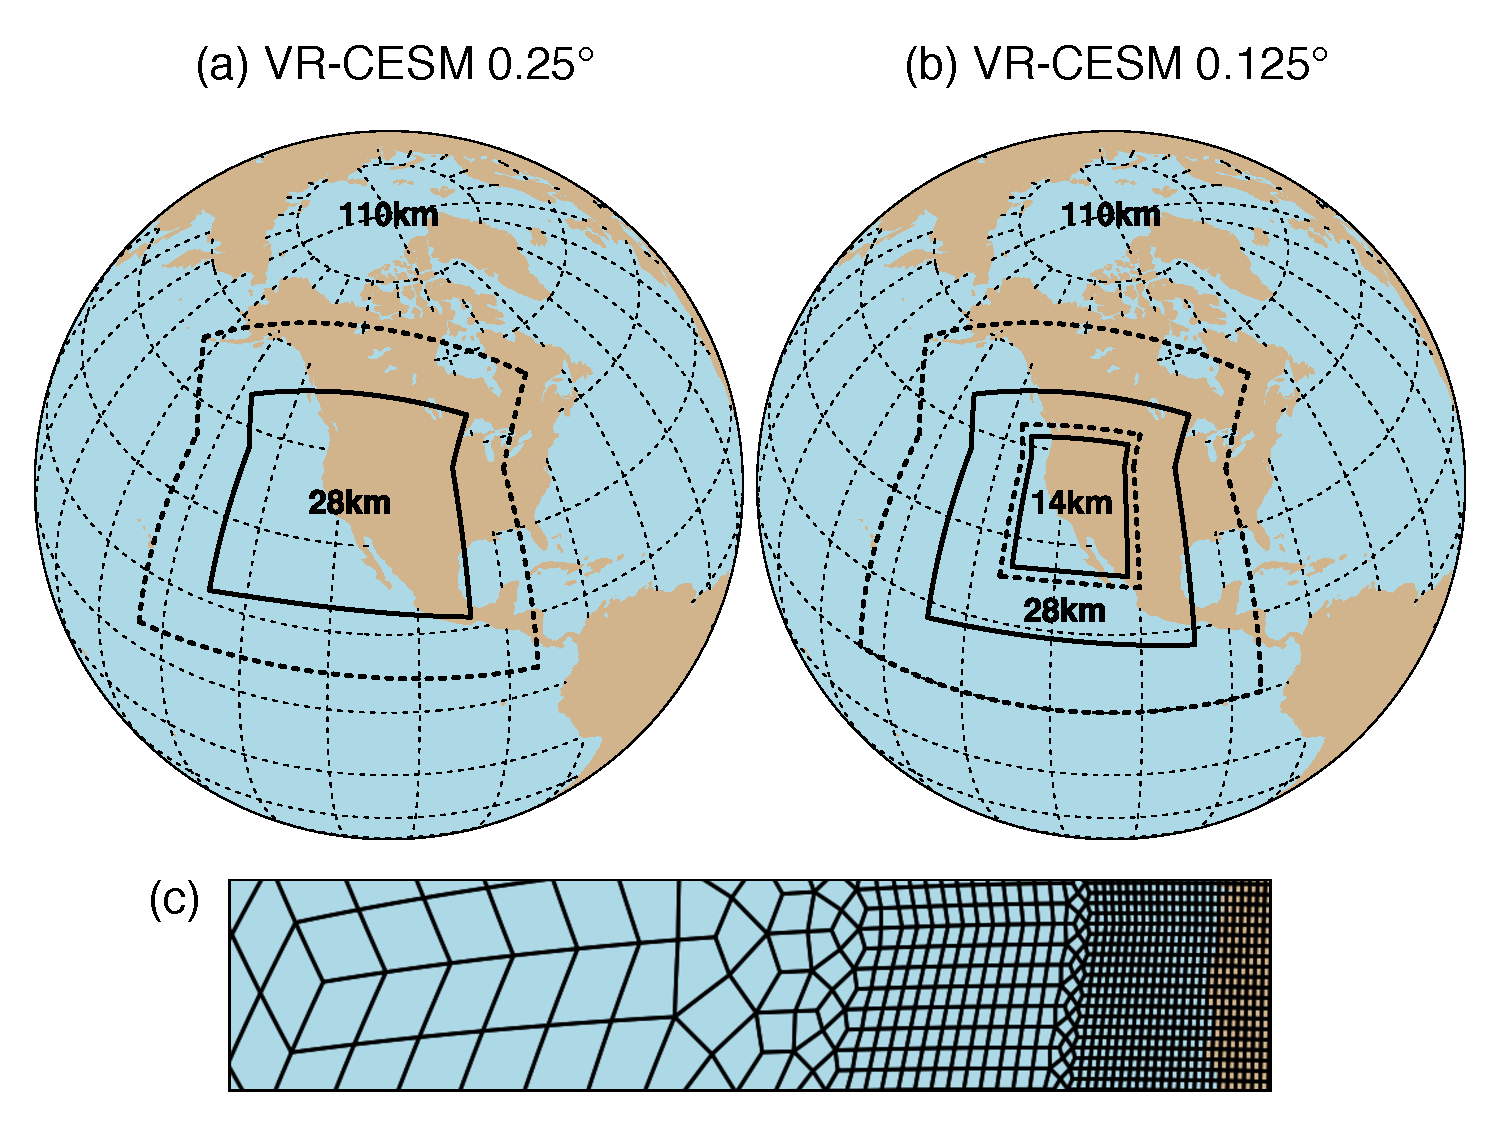
\includegraphics[width=6in]{worldmap_modified.pdf}
\caption{The approximate grid spacing in the (a) VR-CESM 0.25$^\circ$ and (b) VR-CESM 0.125$^\circ$ meshes used in this study. (c) A depiction of the transition from the global $1^\circ$ resolution mesh through two layers of refinement to $0.25^\circ$ and again to $0.125^\circ$.}
\label{fig:Figure 1}
\end{center}
\end{figure}


%Figure 2
\begin{figure}
\begin{center}
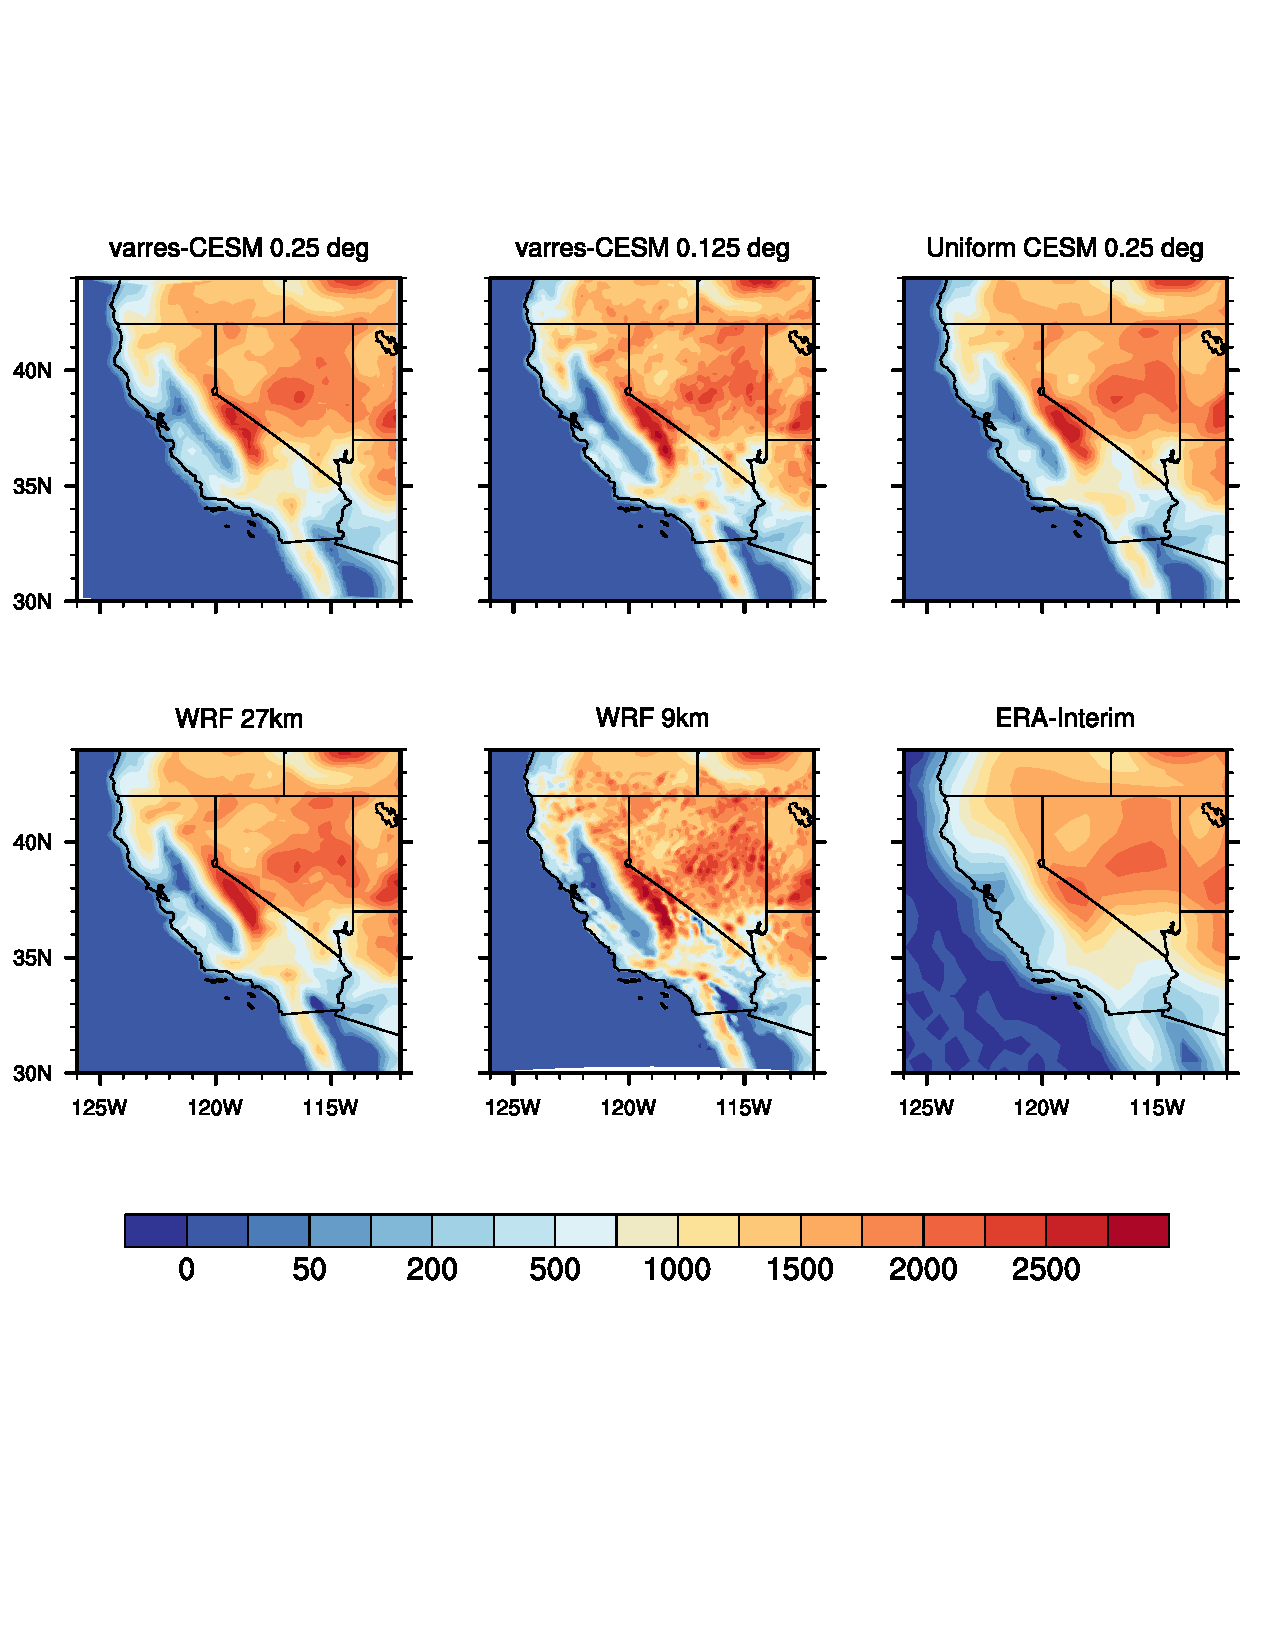
\includegraphics[width=6in]{topo.pdf}
\end{center}
\caption{Upper panel: Topographic heights (from top left to bottom right) for VR-CESM 0.25$^\circ$, VR-CESM 0.125$^\circ$, uniform CESM 1$^\circ$, WRF 27km, WRF 9km, ERA-Interim ($\Delta x \sim$80 km) and USGS ($\sim$3 km); Lower panel: Hypsometric curves for the above datasets.} \label{fig:Figure 2} 
\end{figure}

%Figure 3
\begin{figure}
\begin{center}
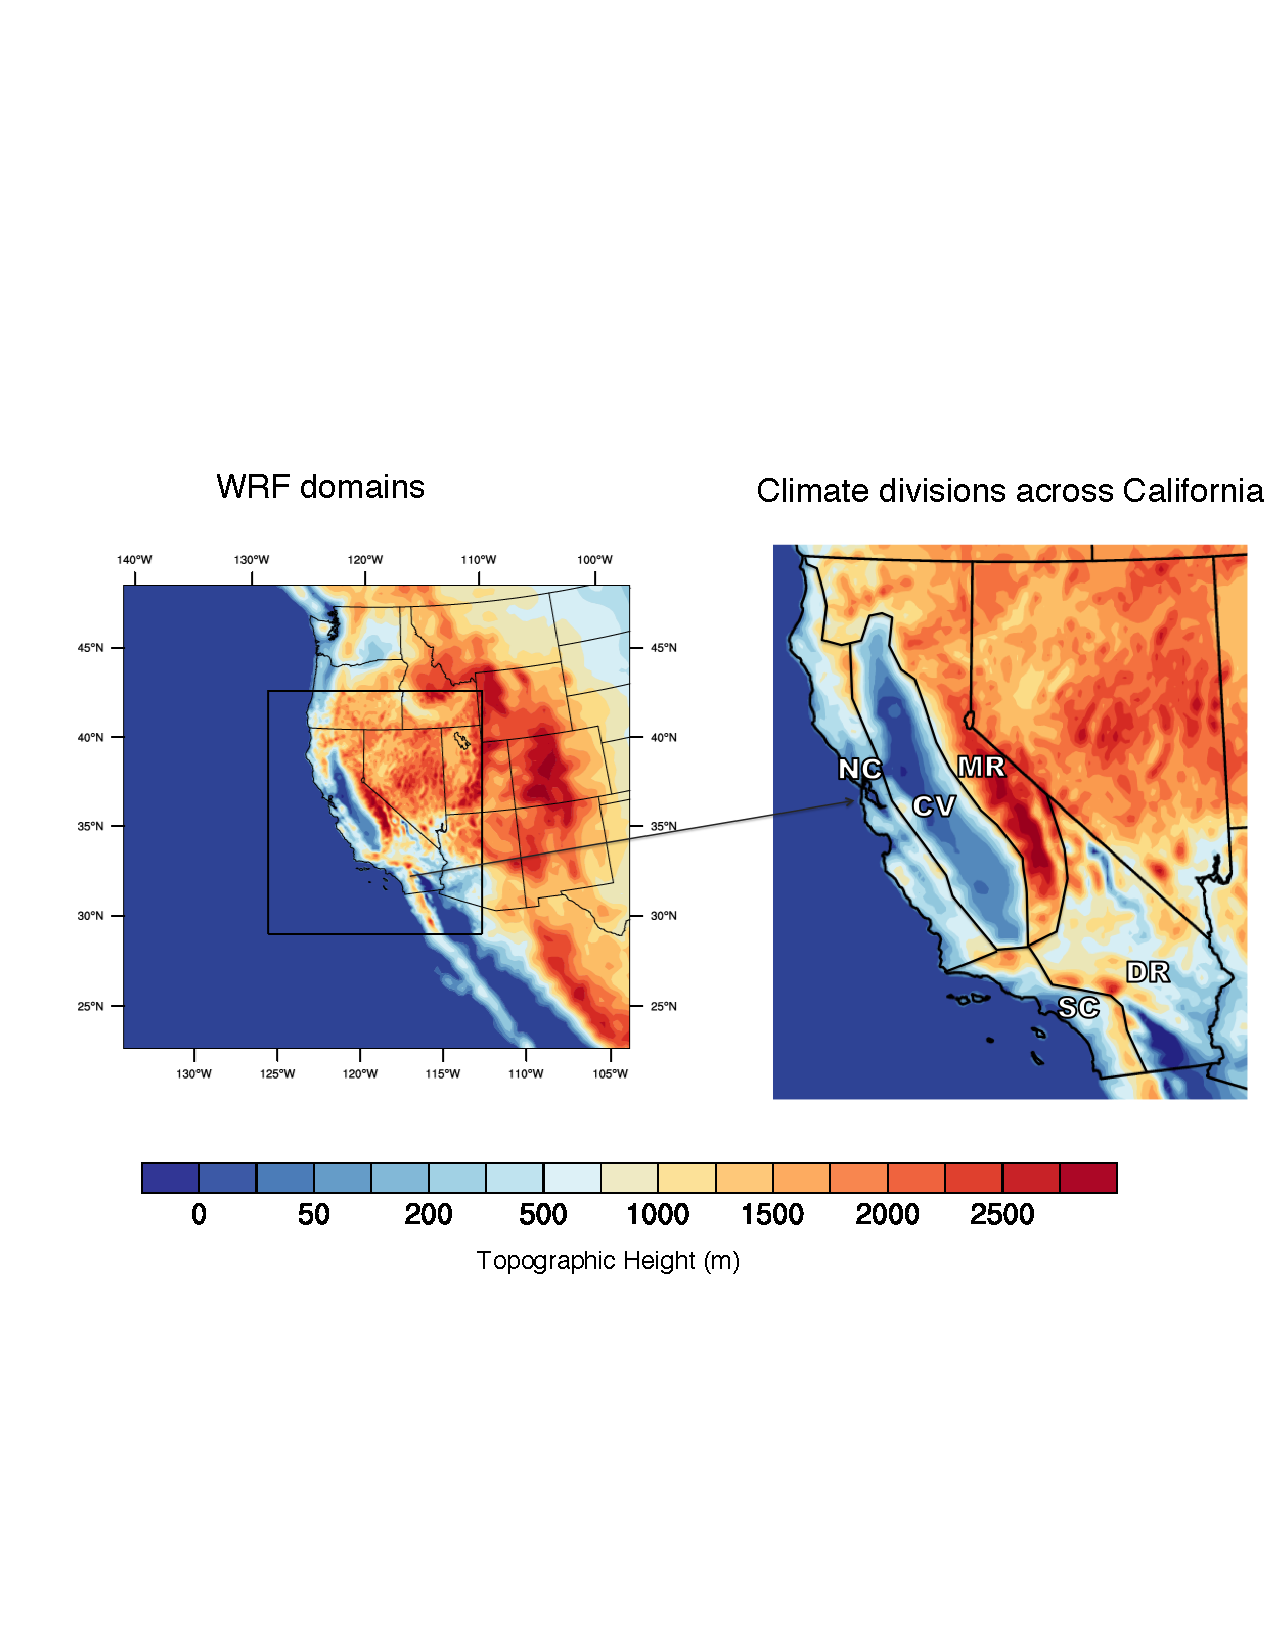
\includegraphics[width=6in]{wrf_domains.pdf}
\end{center}
\caption{Left: WRF 27km (entire plot region) and WRF 9km (solid black box) simulation domains; Right: five climate divisions for California.  Both plots are overlaid with WRF model topography.} \label{fig:Figure 3}
\end{figure}

%Figure 4
\begin{figure}
\begin{center}
\includegraphics[width=6in]{t2_JJA.pdf}
\end{center}
\caption{JJA averaged daily T$_{max}$, T$_{min}$ and T$_{avg}$ from models and reference datasets, and differences (sharing the same legend) between model results and PRISM.} \label{fig:Figure 4}
\end{figure}


%Figure 5
\begin{figure}
\begin{center}
\includegraphics[width=6in]{t2_JJA_std.pdf}
\end{center}
\caption{Sample standard deviation of JJA average daily T$_{max}$, T$_{min}$ and T$_{avg}$ from model results and PRISM.} \label{fig:Figure 5}
\end{figure}

%Figure 6
\begin{figure}
\begin{center}
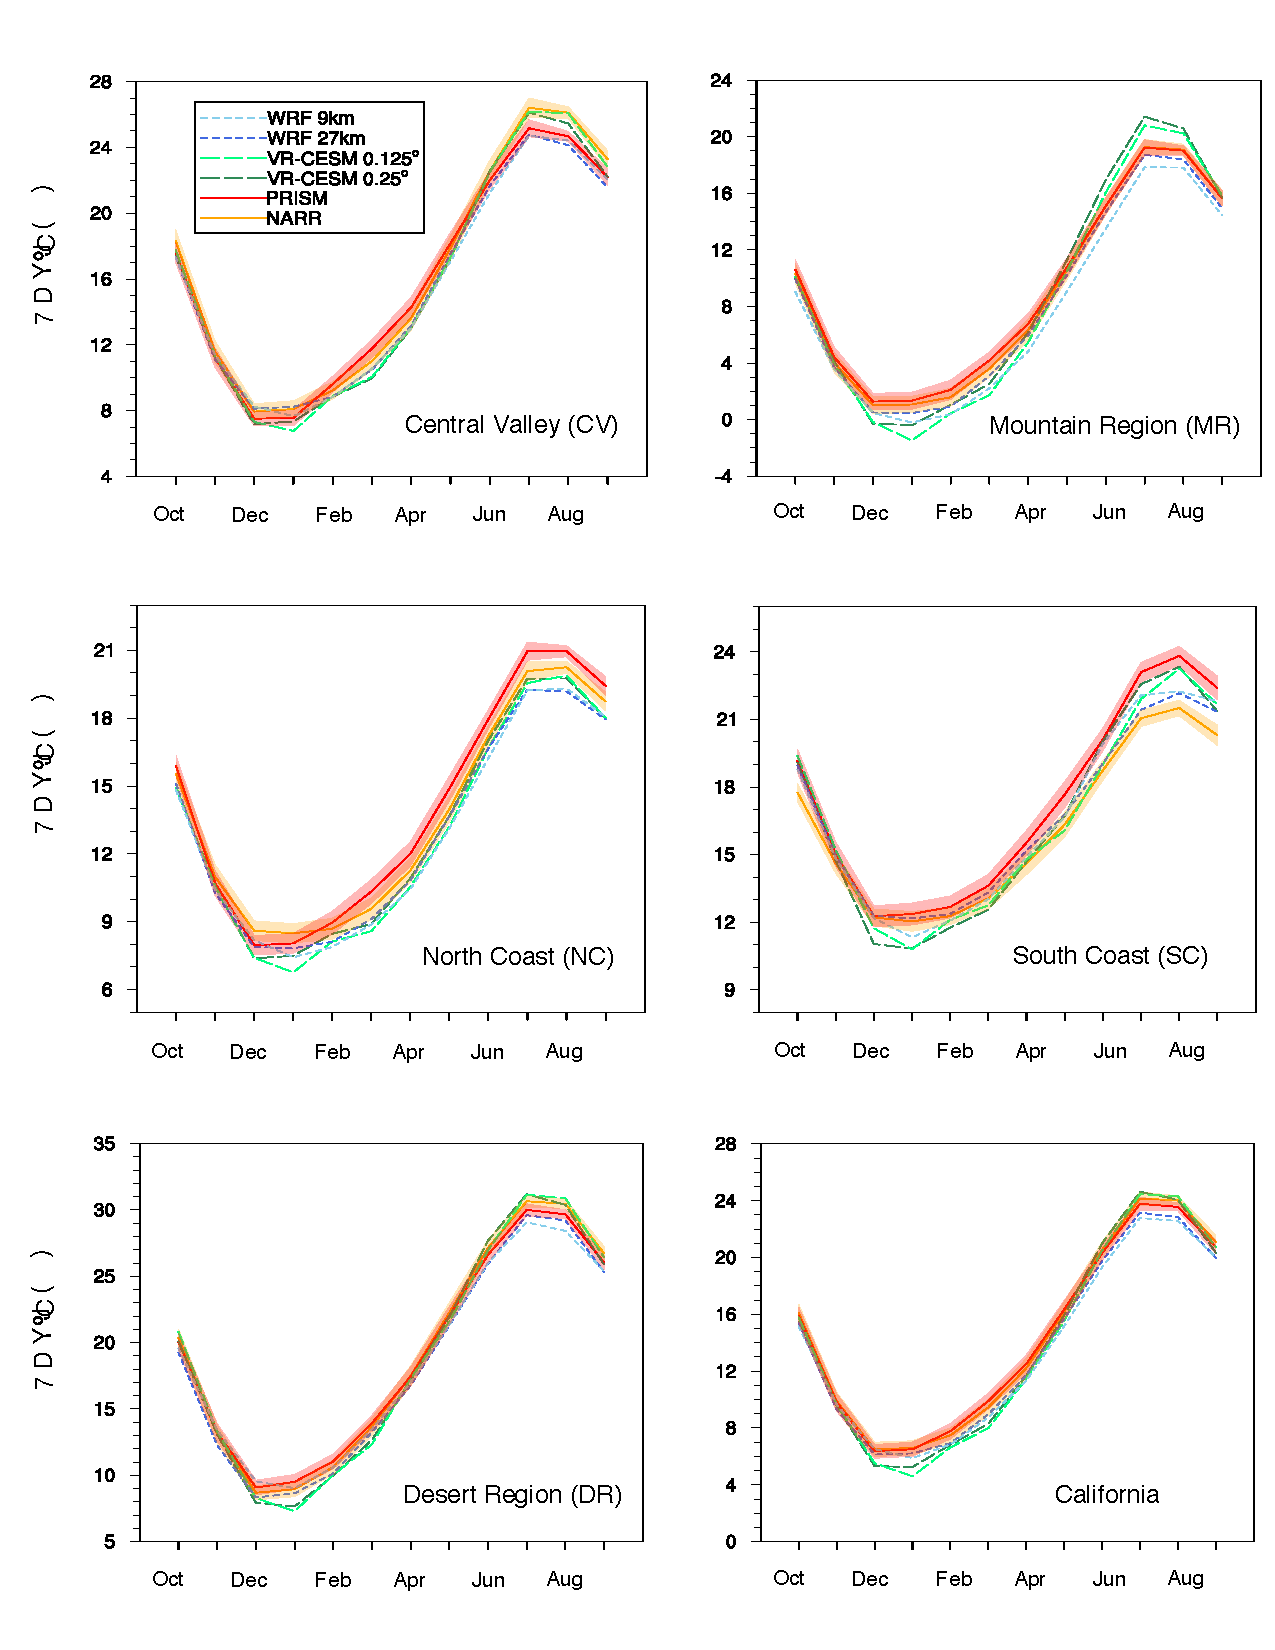
\includegraphics[width=6in]{trd_t2avg_allzones.pdf}
\end{center}
\caption{Seasonal cycle of monthly-average T$_{avg}$ for each climate division. The shading corresponds to the 95\% confidence interval of PRISM and NARR. } \label{fig:Figure 6}
\end{figure}

%Figure 7
\begin{figure}
\begin{center}
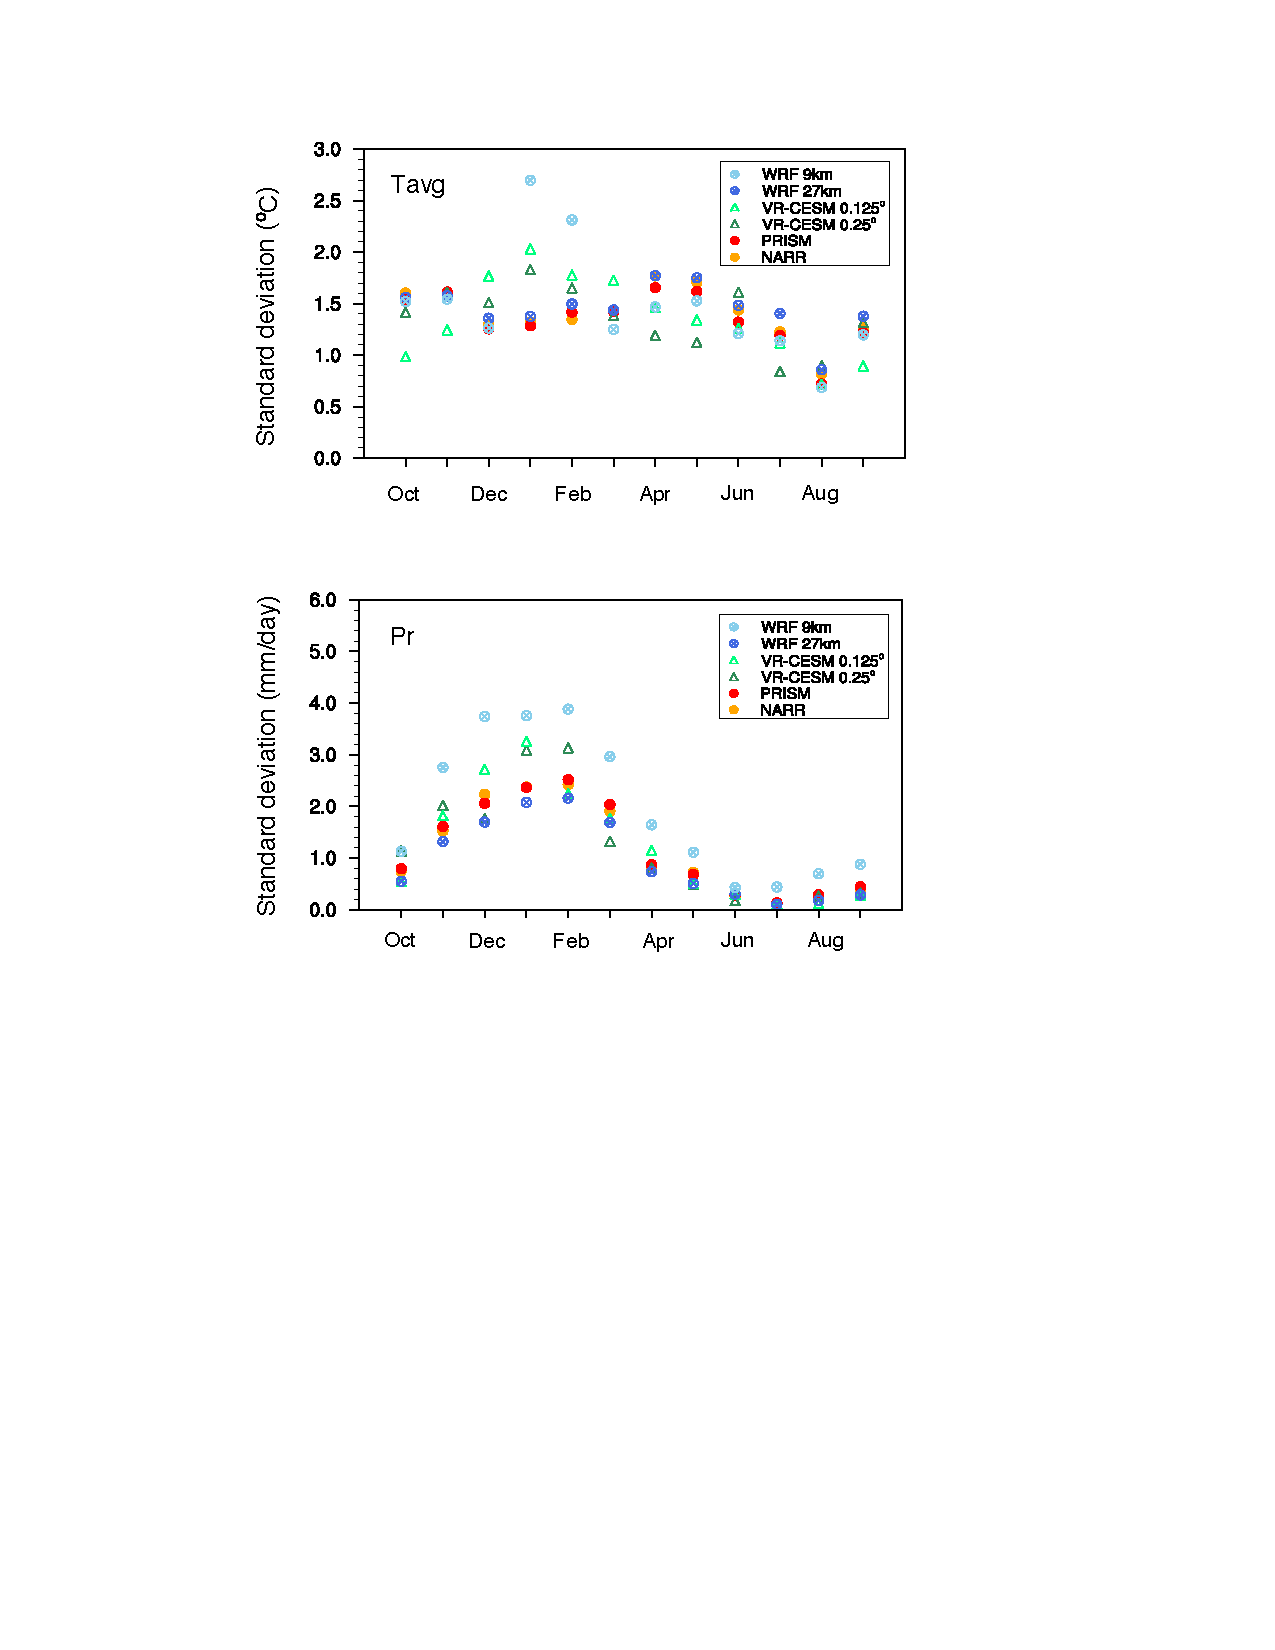
\includegraphics[width=6in]{trd_t2avg_pr_std.pdf}
\end{center}
\caption{Standard deviation values of monthly-average T$_{avg}$ and Pr averaged over California.} \label{fig:Figure 7}
\end{figure}

%Figure 8
\begin{figure}
\begin{center}
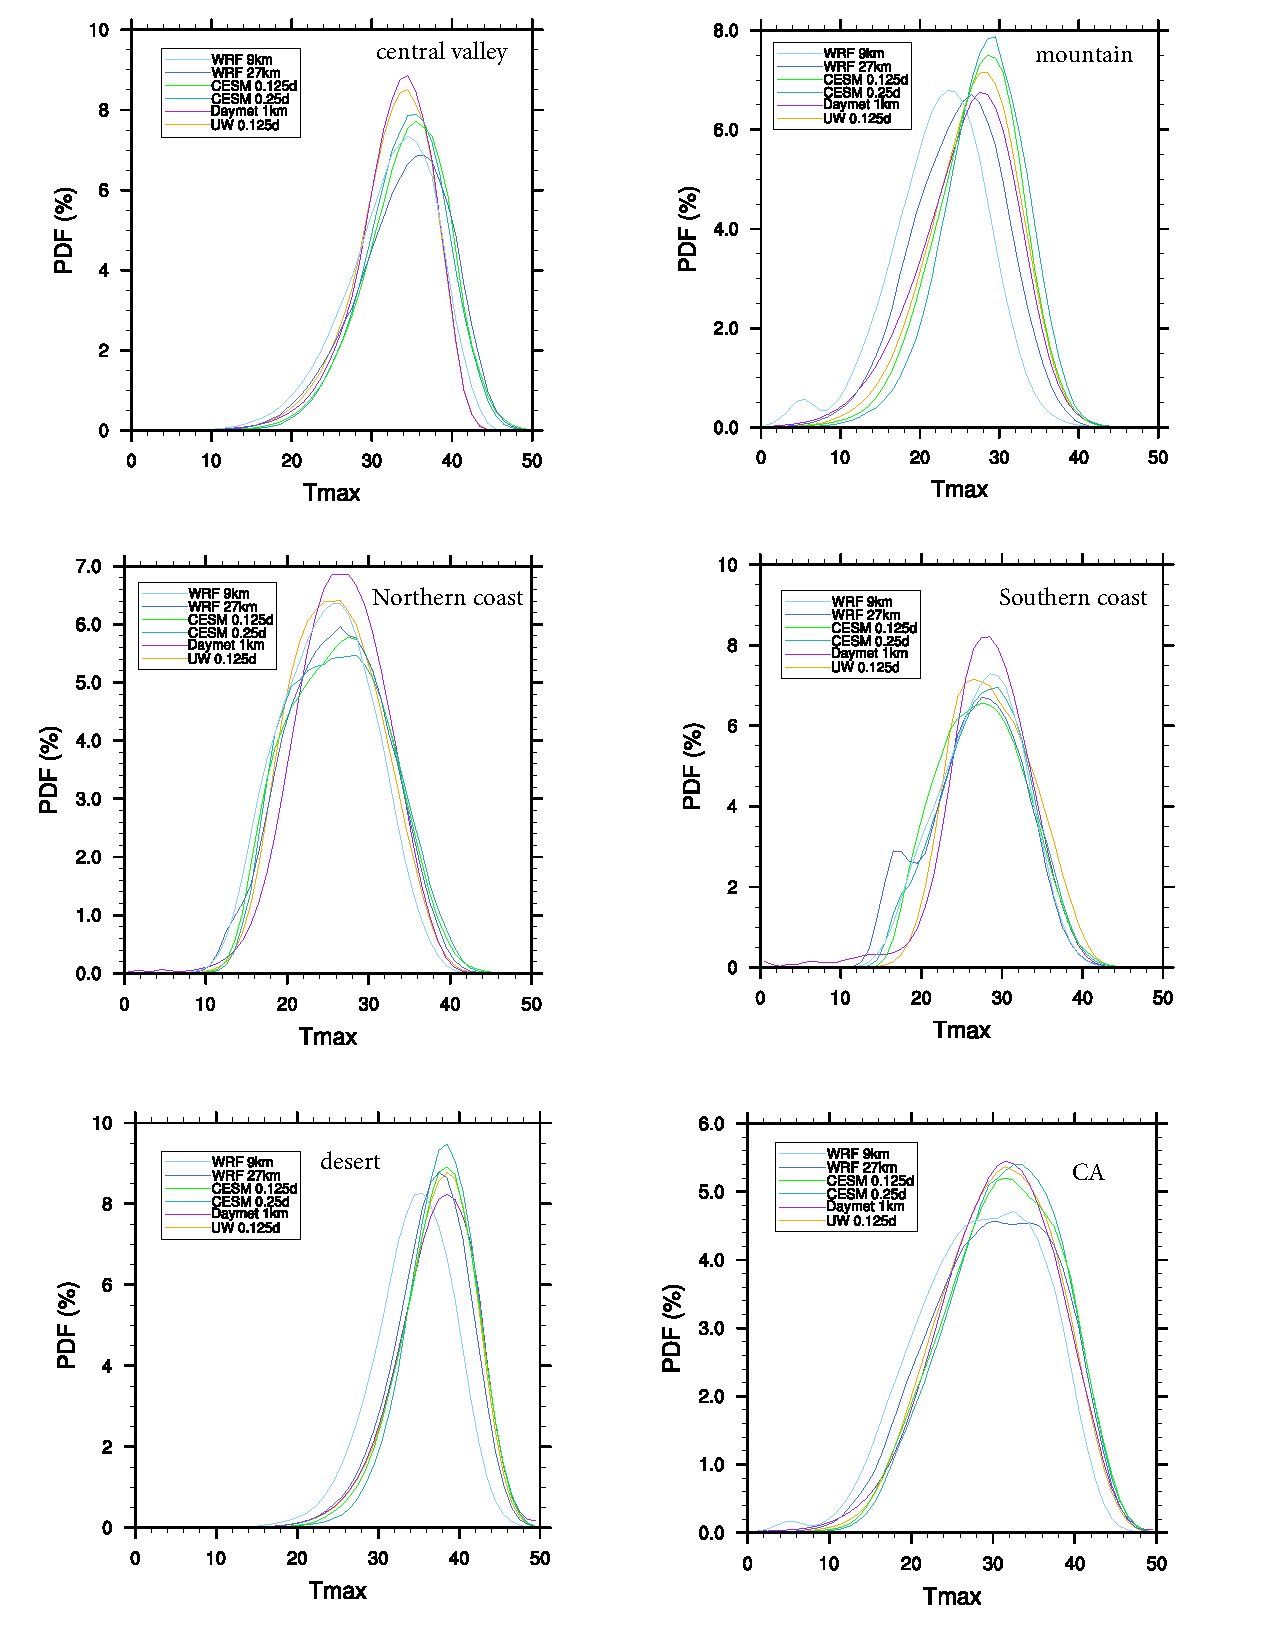
\includegraphics[width=6in]{PDF_t2max_allzones_JJA.pdf}
\end{center}
\caption{Frequency distribution of JJA daily T$_{max}$ over the simulation period 1980-2005.} \label{fig:Figure 8}
\end{figure}

%Figure 9
\begin{figure}
\begin{center}
\includegraphics[width=6in]{pr_DJF_Annual.pdf}
\end{center}
\caption{Annual and DJF precipitation from model results and reference datasets, absolute/relative differences between model results and PRISM.} \label{fig:Figure 9}
\end{figure}

%Figure 10
\begin{figure}
\begin{center}
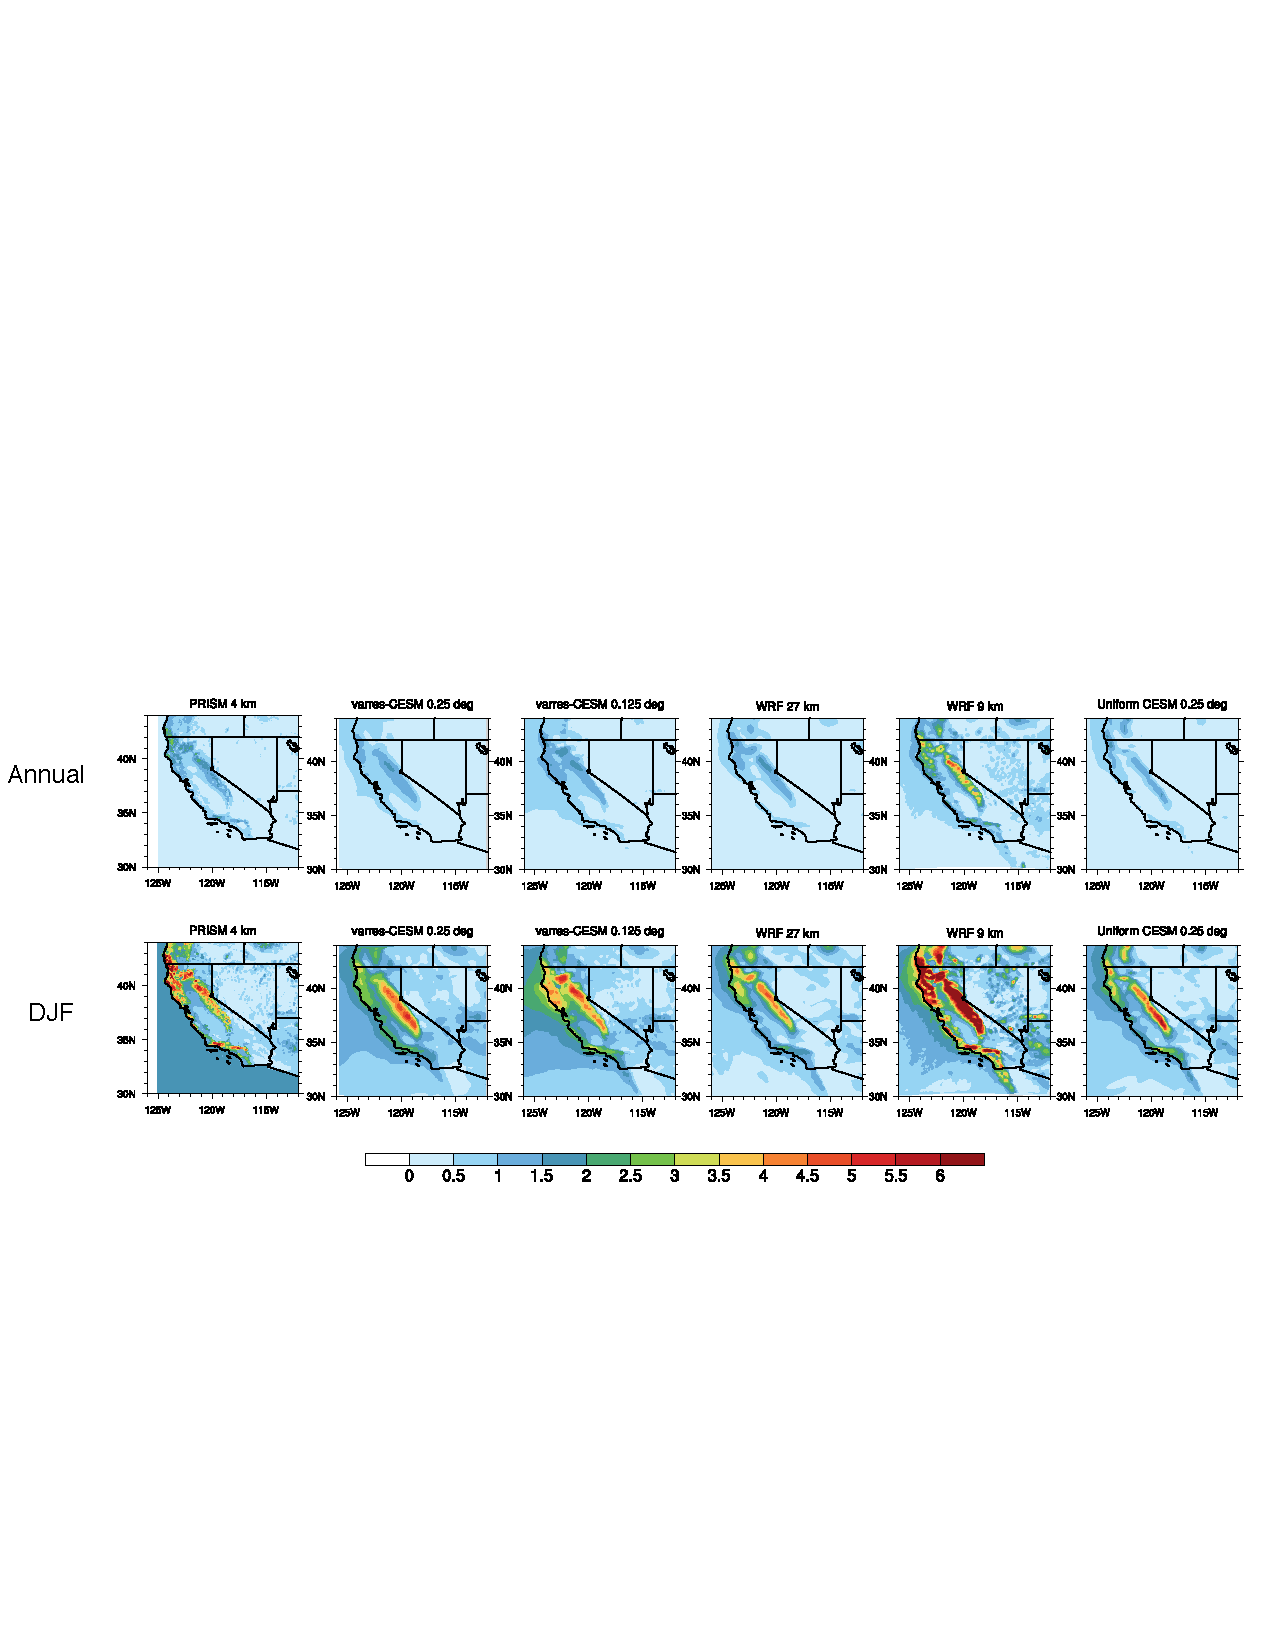
\includegraphics[width=6in]{pr_DJF_Annual_std.pdf}
\end{center}
\caption{Sample standard deviation of Annual and DJF precipitation from models and PRISM.} \label{fig:Figure 10}
\end{figure}

%Figure 11
\begin{figure}
\begin{center}
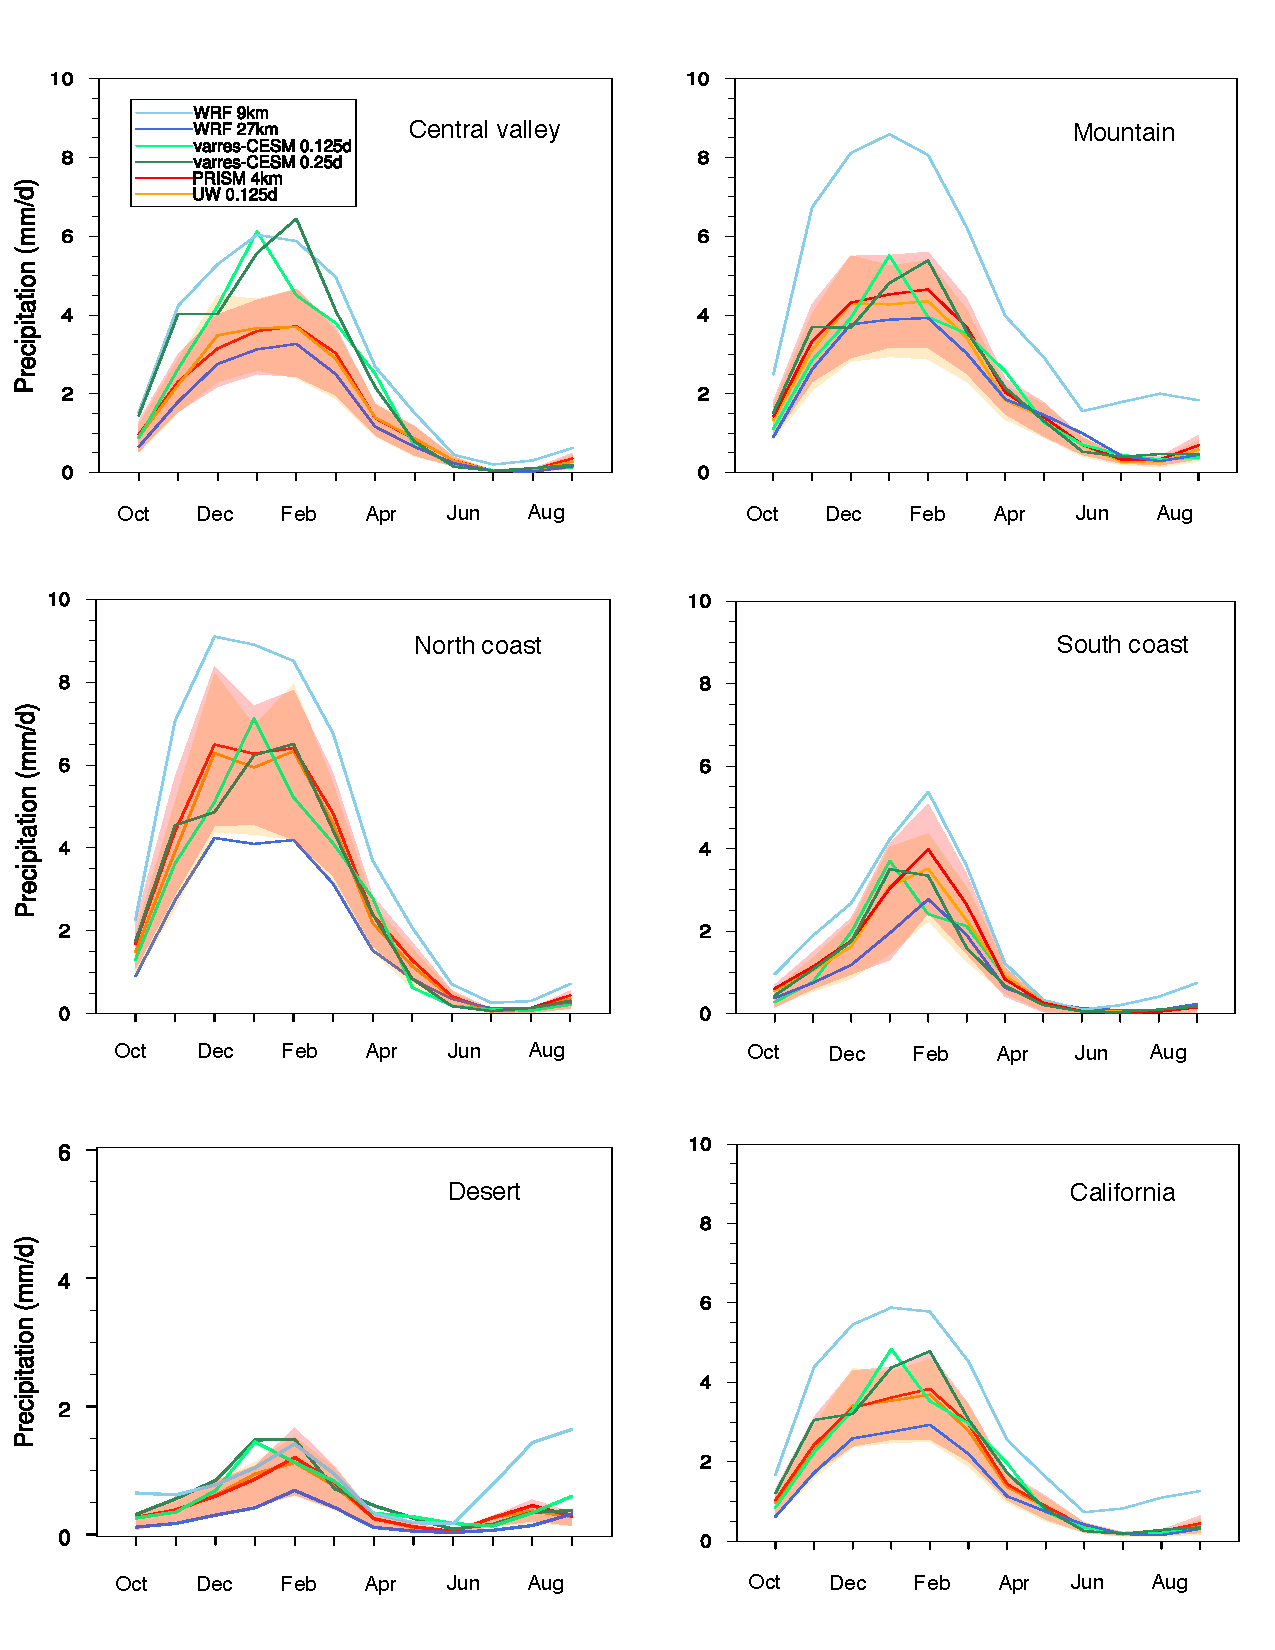
\includegraphics[width=6in]{trd_pr_allzones.pdf}
\end{center}
\caption{As Figure 6, but for monthly-average total precipitation. The shading refers to the 95\% confidence interval of PRISM and UW.} \label{fig:Figure 11}
\end{figure}


%%Figure 12
%\begin{figure}
%\begin{center}
%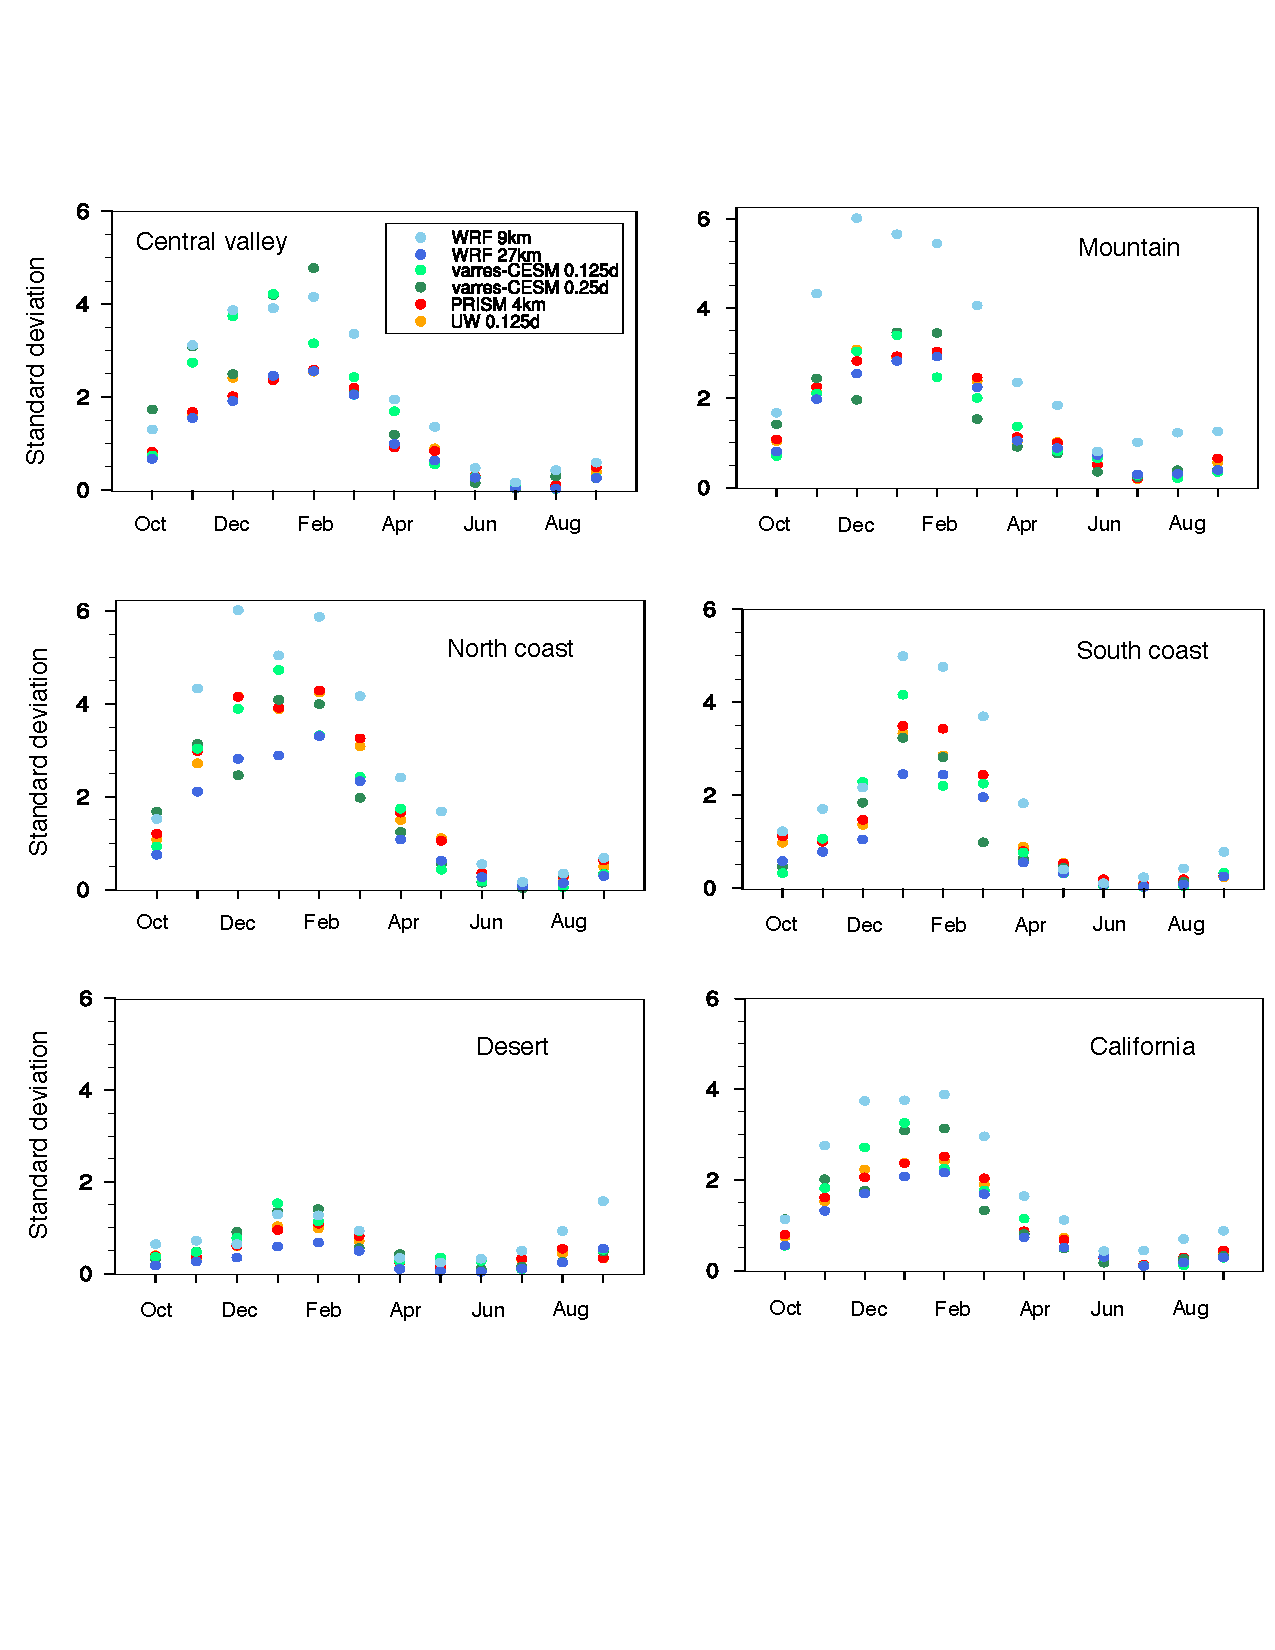
\includegraphics[width=6in]{trd_pr_allzones_std.pdf}
%\end{center}
%\caption{As Figure 7, but for monthly-average total precipitation.} \label{fig:Figure 12}
%\end{figure}

%Figure 13
\begin{figure}
\begin{center}
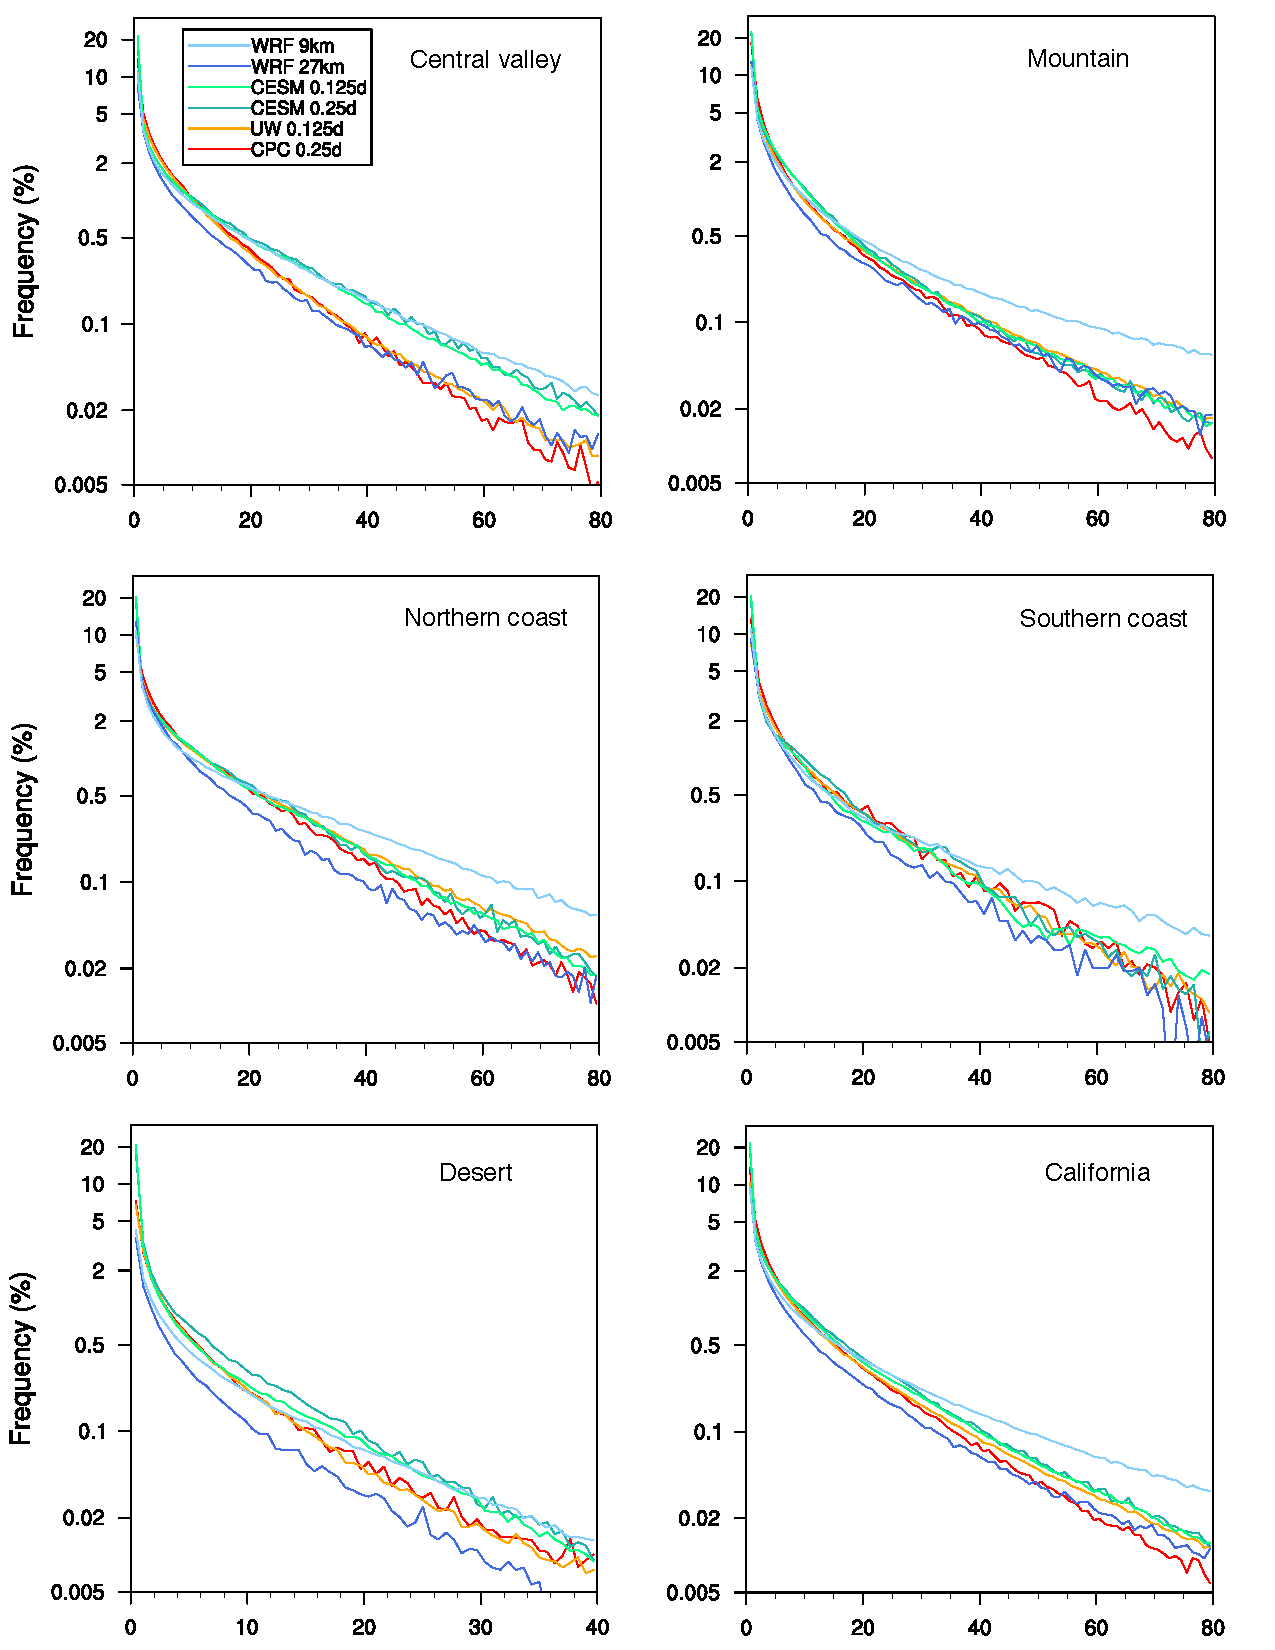
\includegraphics[width=6in]{PDF_pr_allzones_DJF.pdf}
\end{center}
\caption{As Figure 8, but for DJF rainy days (Pr$>=$0.1mm$/$day) (note that the vertical scale is logarithmic).} \label{fig:Figure 13}
\end{figure}

%Figure 14
%\begin{figure}
%\begin{center}
%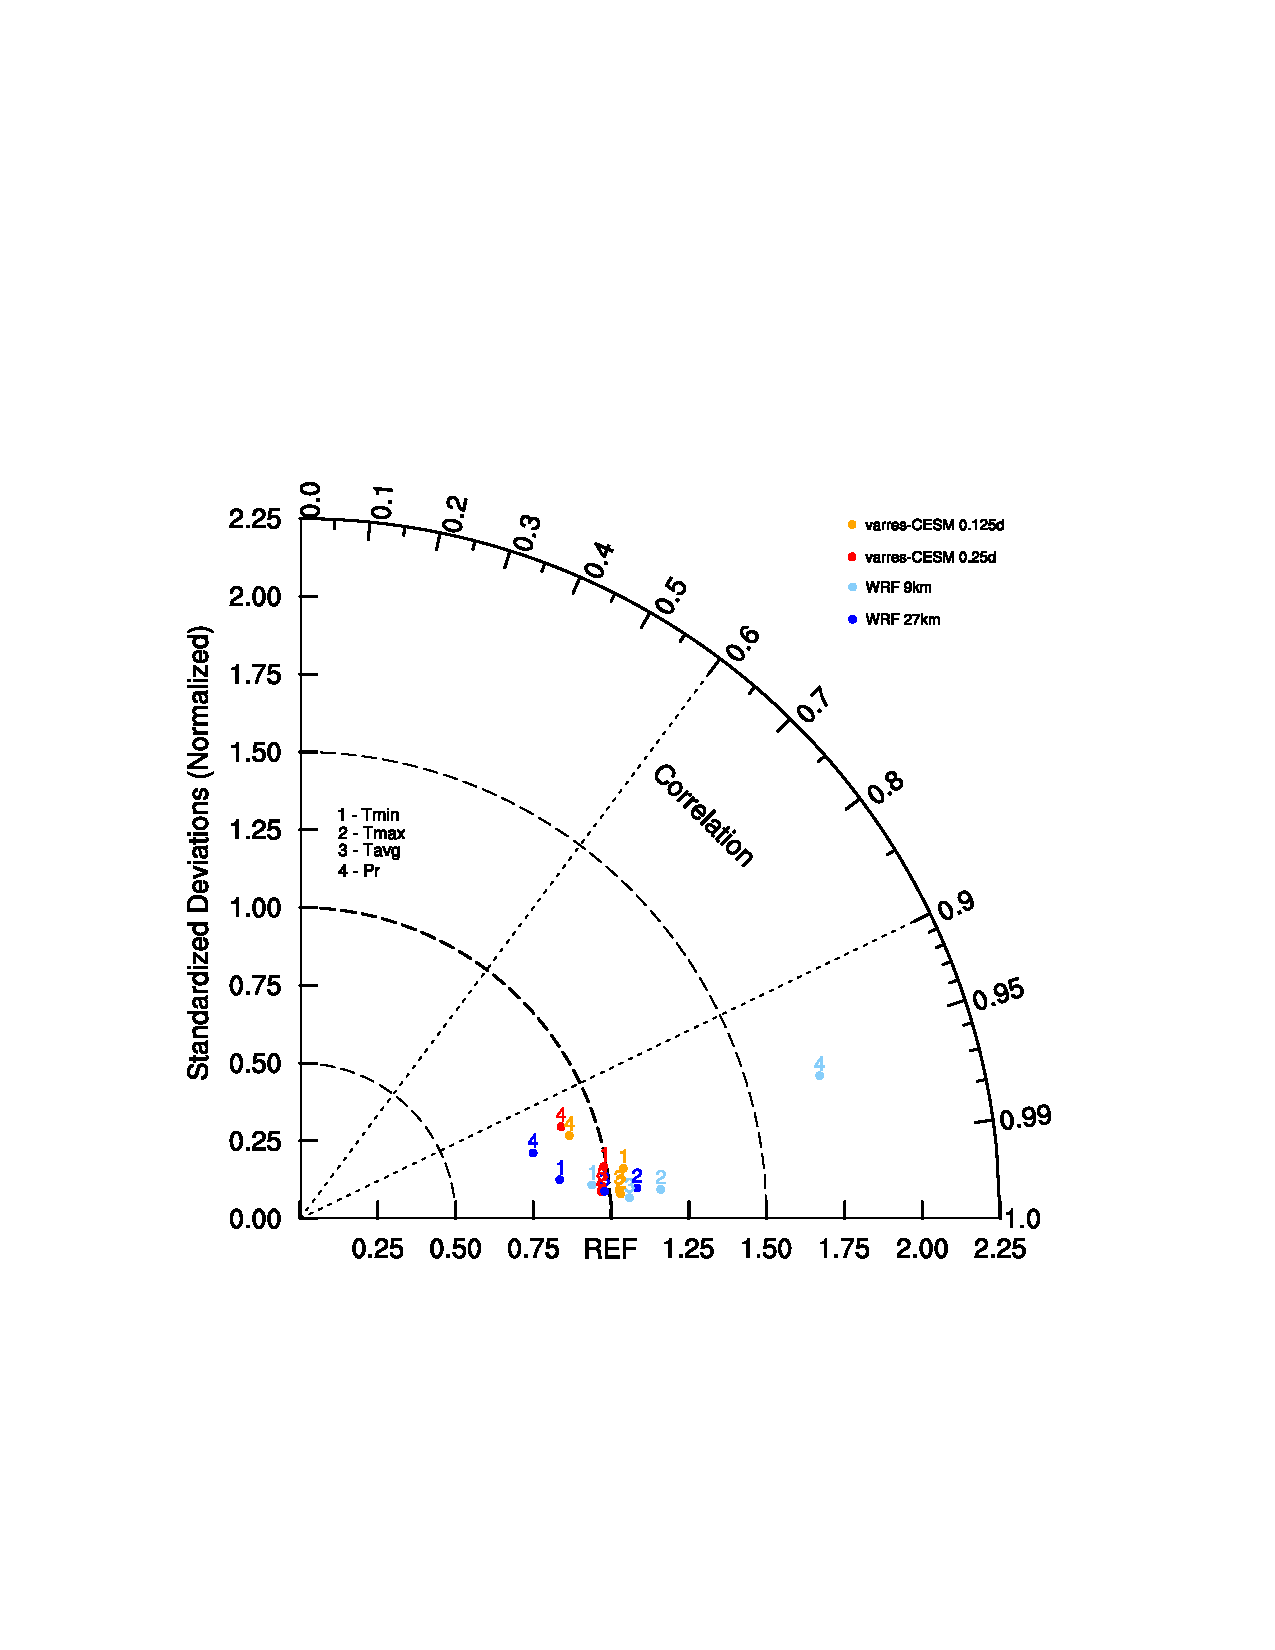
\includegraphics[width=6in]{taylor_diagram.pdf}
%\end{center}
%\caption{Taylor diagram of the annual climatology for the entire California region using the PRISM dataset as reference.} \label{fig:Figure 14}
%\end{figure}

%new Figure
\begin{figure}
\begin{center}
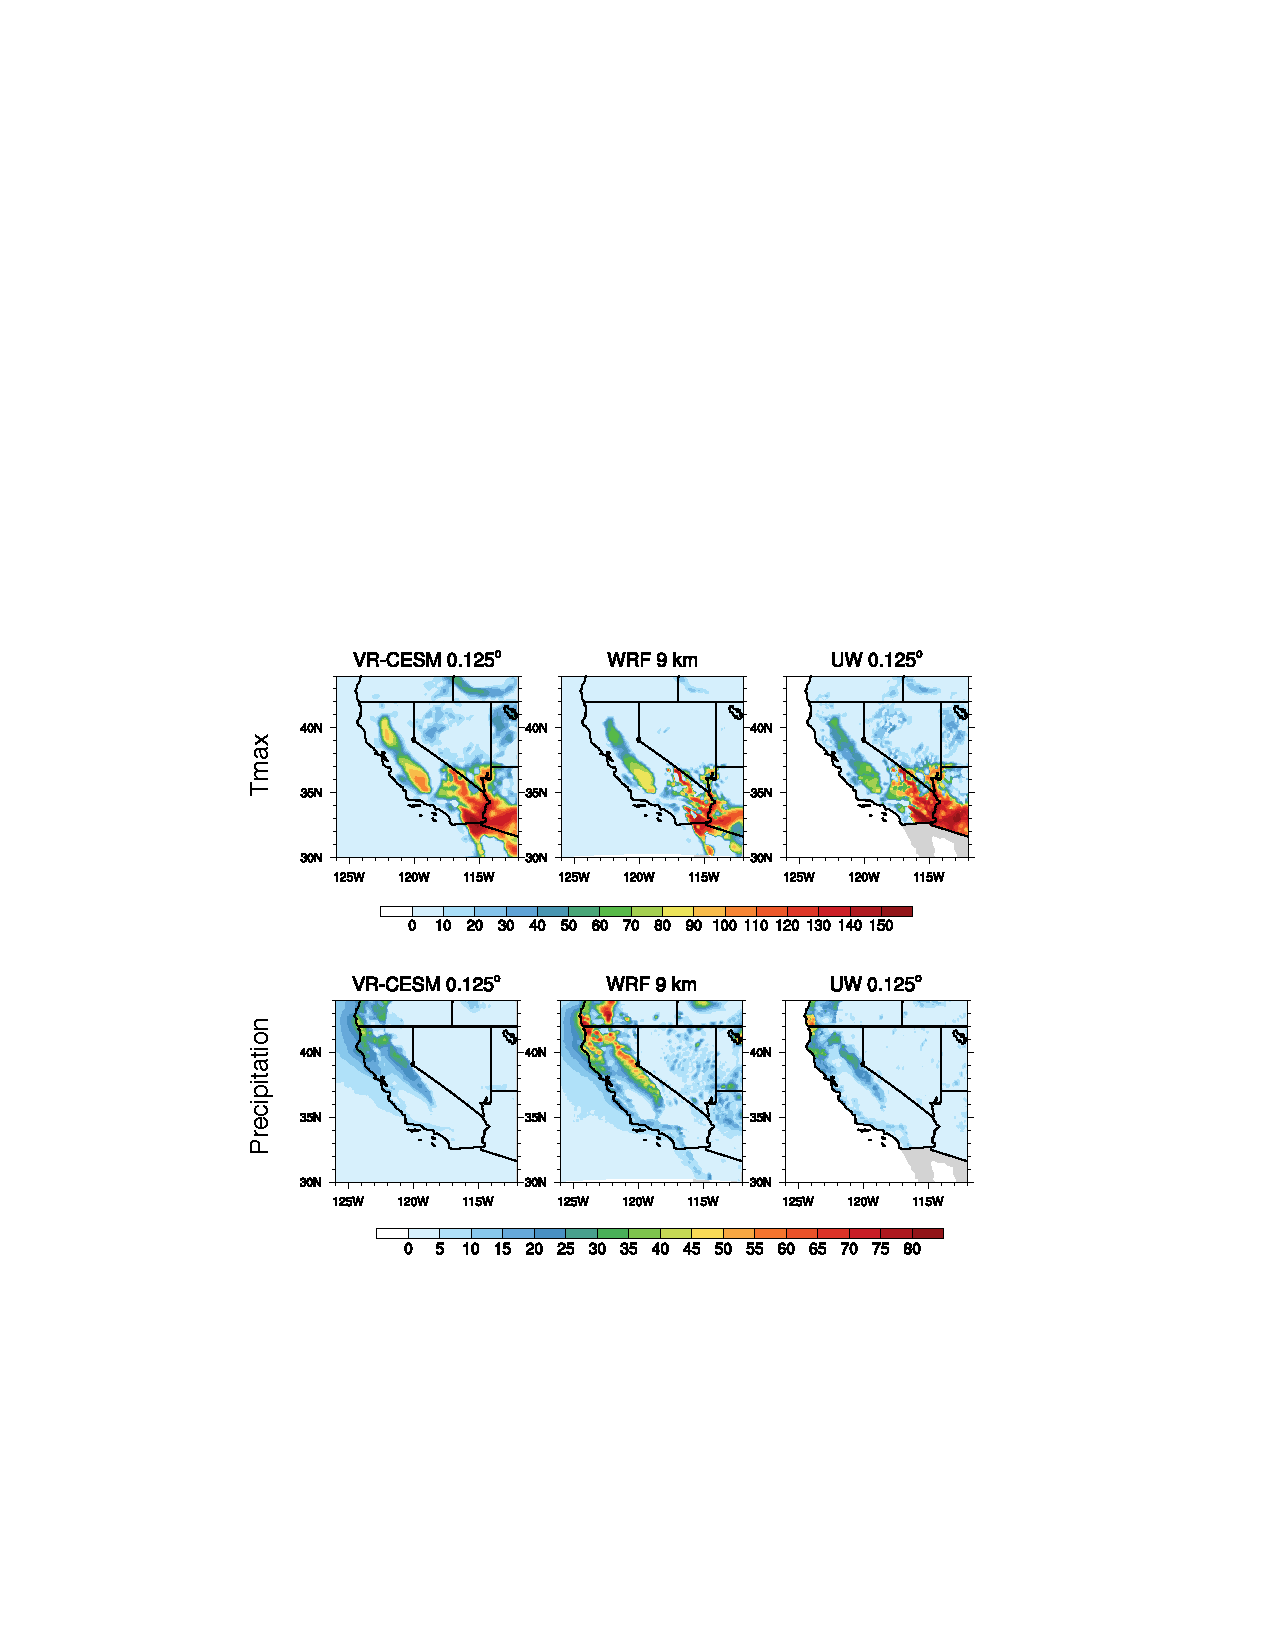
\includegraphics[width=6in]{t2max>35_pr>20.pdf}
\end{center}
\caption{Number of days per year with (top) T$_{max}$$>$35$^\circ$C and (bottom) Pr$>$20mm/day in VR-CESM 0.125$^\circ$, WRF 9km and UW over the simulation period 1980-2005.} \label{fig:Figure 15}
\end{figure}



\end{document}
